\section{Result}
\label{sec:result}

\subsection{Experiment environment}
We implement ZomeFab in C++ and Python on desktop PC with 3.4GHz CPU and 16GB memory. 
% The assembling processes are showed in Table \ref{tab:result_ZomeFab_real}. 
% The inner structure is built by Zometool which can construct a strong structure easily. 
The outer surfaces are printed by Ultimaker 3, a low-cost FDM 3{D} printer with 0.2m x 0.2m x 0.2m printing volume and PLA material. 
The time it takes to assemble the fabricated parts for these objects range from few minutes to around an hour, depending on the number of parts.

\subsection{Evaluation}
We evaluate the material cost and fabrication time between ``Zomefab" and solid-printed object (denoted as ``baseline" method).
% with simple partition method. 
We use CURA~\cite{cura}, a slicer software for 3{D} printing, to simulate the fabrication time and used materials for solid-printed object.
Meanwhile, we subdivide the shape using a octree, and stop the subdivision once each sub-shape fit into the printing volume.
% The software will evaluate the fabrication time and the a amount of materials if the volume of input mesh is printable.
To evaluate our method, we report two different infill methods called ``hollow" and ``solid".
Shapes printed under ``hollow" use only 20\% infill rate, where ``solid" use 100\% infill rate.
Note that we only use 20\% infill rate to fabricate the results shown in this paper, and the ``solid" results are simulated using CURA.
% As shown in \tabname~\ref{tab:result_material}, our method greatly saves materials from 24\% to 64\% under ``hollow" setting, and from 68\% to 85\% under ``solid" setting.
% As expected that our method brings more benefits when infill rate grows.
% In terms of fabrication time evaluation, we report both single 3D printer scenario and multiple 3D printer scenario.
% In multiple 3D scenario, we assume there are enough 3D printers so that we can print all pieces simultaneously.

% As reported in \tabname~\ref{tab:result_material} and \tabname~\ref{tab:result_time}, our method saves 
% we evaluate 
% four configurations for each object:
% \begin{itemize}
%     \item hollow-printed with 20\% infill
%     \item solid-printed using Zomefab
%     \item 
% \end{itemize}
% demonstrate four experiments for each object, print hollowed with 20\% infill and print solid by Zomefab and baseline that partitions a solid object into 3D printable parts. \\
% The experiment assumes two conditions: 
% \begin{enumerate}
% \item Baseline is that it prints input mesh as pieces and use 3D printer only. (We use octree for segmentation)
% \item In multiple 3{D} printer experiment, we have enough  3D printers like the maker’s studio that we can print all pieces simultaneously. 
% \end{enumerate}
% The following paragraph will discuss the material cost and the printing time.

\subsubsection{Material cost}
As shown in \tabname~\ref{tab:result_material}, our method greatly saves materials from 24\% to 64\% under ``hollow" setting, and from 68\% to 85\% under ``solid" setting.
As expected that our method brings more benefits when infill rate grows.
The material cost are listed as follow: 0.56 USD/meter (Ultimaker official PLA material price), Zometool rod: 0.19 USD/rod and Zome-ball: 0.29 USD/ball (Zometool official price) for our experiments. 
% Material cost sets printing material: 0.56 USD/meter (Ultimaker official PLA material from official online shop, 90 meters sell 50 USD), Zometool rod: 0.19 USD/rod (from Zometool official online shop, 100 rods sell 19 USD) and Zome-ball: 0.29 USD/ball (from Zometool official online shop, 100 Zome-balls sell 29 USD) for our experiments. 
% In Table \ref{tab:result_material}, all of experiments show that our method cost less material than baseline. Even if we print the result in 20\% fill rate, we also saved about 25\% of the material cost.

\subsubsection{Printing time}
We report printing time evaluation under both single 3D printer scenario and multiple 3D printer scenario.
In multiple 3D scenario, we assume there are enough 3D printers so that we can print all pieces simultaneously.
In Table \ref{tab:result_time}, we demonstrate the statistical comparison of printing time between single 3{D} printer and multiple 3{D} printers. 
In single 3{D} printer scenario, the fabrication time of our method under ``hollow" configuration is longer than the baseline method.
The main reason is because the pieces of baseline method fit the printing volume better (regularly cutted), where the printing paths can be optimized without the time waste on printing redundant support materials.
And the pieces of our method is highly non-regular with connectors, so the printing paths is more complicated compare to baseline pieces.
Note that as the infill rate grows, we can discover that the growing rate of our method is way less than the baseline method, and is able to save from 52\% to 68\% of printing time.
% the fabrication time is more than baseline in 20\% infill rate. We propose that our mesh's complexity is higher than baseline testing mesh. 
In multiple 3{D} printers scenario, we assume that we have enough 3{D} printers, so the reported time of our method is the longest printing time among all pieces.
% our method just has to wait the piece which has the most printing time. 
The statistics shows that our method printing time is absolutely faster than baseline in different fill rate using multiple 3{D} printers. 
% It demonstrates that our method's printing time will decrease if user can use more 3{D} printers. (See \figname~\ref{fig:multi_printer}) 
If the user just has single 3{D} printer and wants to get a exquisite result, our method can also get lower cost and fabrication time.

\subsection{Zometool Use}
Table \ref{tab:result_Zometool} shows the quantity of Zometool rods and balls used in each result. 
In \secname~\ref{sec:Zometool}, we use smallest blue rods to make the zome-cube as the unit structure in order to make the best-fit initial structure. 
The bigger the object is, more smallest blue rods (${b_0}$) will be used.
We also observed that, blue rods and yellow rods are more likely to be used interchangeably since we encourage regularity during  simulated annealing optimization. 
% So the number of smallest yellow rods will increase if we use more smallest blue rods.
Meanwhile, the rule of Zometool indicates that the longest rod only can be replaced by one shortest and middle rod in the same color.
So it seldom introduce red rods into the structure, which resulted in the used number of rods imbalance shown in \tabname~\ref{tab:result_Zometool}.
% Also, Zometool components has some special relationships between each of them: 
% \begin{itemize}
% \item The blue rods and yellow rods are more compatible than the blue rods and red rods. 
% \item The longest rod only can be replaced by one shortest and middle rod in the same color.
% \end{itemize}

Except the smallest yellow and blue rods, the other rods are used few or none in our simulated annealing rule.
%The red rods, middle rods and long rods in all colors used few or none in our simulated annealing rule.

\begin{table*}[ht]
\centering
\resizebox{1.\linewidth}{!} {
\begin{tabular}{|c|c|c|c c c|c|} \hline
 \multirow{2}*{Mesh} & \multirow{2}*{Infill Method} & \multirow{2}*{Fabrication Method} & \multicolumn{3}{c|}{Material Cost (USD)} & Efficiency (Saved)\\\cline{4-7} 
 & & & 3D printing & Zometool & Overall (sum) & Material \\ \hline
 
 \multirow{4}*{Moai} & \multirow{2}*{Hollow} & Zomefab & 82.56 & 70.57 & 153.13  & \multirow{2}*{13.83\%} \\ 
 &  & Baseline & 177.71 &  & 177.71 &\\\cline{2-7}
 & \multirow{2}*{Solid} & Zomefab & 170.9 & 70.57 & 241.47  & \multirow{2}*{65.11\%} \\
 &  & Baseline & 692.07 & & 692.07 &\\ \hline
  
 \multirow{4}*{Squirrel} & \multirow{2}*{Hollow} & Zomefab & 100.38 & 77.55 & 177.93 & \multirow{2}*{64.67\%} \\ 
 &  & Baseline & 503.56 & & 503.56  &\\\cline{2-7}
 & \multirow{2}*{Solid} & Zomefab & 213.96 & 77.55 & 291.51  & \multirow{2}*{85.42\%}\\
 &  & Baseline & 2000.00 & & 2000.00 &\\ \hline
 
 \multirow{4}*{Doraemon} & \multirow{2}*{Hollow} & Zomefab & 101.38 & 76.34 & 177.72 & \multirow{2}*{24.43\%}\\ 
 &  & Baseline & 235.16 & & 235.16 &\\\cline{2-7}
 & \multirow{2}*{Solid} & Zomefab & 227.78 & 76.34 & 304.12 &  \multirow{2}*{68.24\%}\\
 &  & Baseline & 957.42 & & 957.42 &\\ \hline
 
\multirow{4}*{Totoro} & \multirow{2}*{Hollow} & Zomefab & 72.32 & 61.48 & 133.80 & \multirow{2}*{27.84\%}\\ 
 &  & Baseline & 185.41 & & 185.41 &\\\cline{2-7}
 & \multirow{2}*{Solid} & Zomefab & 148.26 & 61.48 & 209.74 &  \multirow{2}*{71.17\%} \\
 &  & Baseline & 727.51 & & 727.51 &\\ \hline
 
\multirow{4}*{Iron Man} & \multirow{2}*{Hollow} & Zomefab & 73.99 & 57.76 & 131.75 & \multirow{2}*{34.12\%} \\ 
 &  & Baseline & 199.97 & & 199.97 &\\\cline{2-7}
 & \multirow{2}*{Solid} & Zomefab & 149.67 & 57.76 & 207.43 &  \multirow{2}*{72.93\%} \\
 &  & Baseline & 766.24 & & 766.24 &\\ \hline
 
\end{tabular}
}
\caption{ZomeFab's performance on saving material as compared to a baseline method.}
\label{tab:result_material}
\end{table*}

\begin{table*}[ht]
\centering
\resizebox{1.\linewidth}{!} {
\begin{tabular}{|c|c|c|c c c| c c c|c | c|} \hline
 \multirow{2}*{Mesh} & \multirow{2}*{Infill Method} & \multirow{2}*{Fabrication Method} & \multicolumn{3}{c|}{Single 3{D} Printer Fabrication Time (hours)} & \multicolumn{3}{c|}{Multiple 3{D} Printer Fabrication Time (hours)} & \multicolumn{2}{c|}{Efficiency (Saved)}\\\cline{4-11} 
 & & & 3D printing & Zometool & Overall (sum) & 3D printing & Zometool & Overall (max) & Single & Multiple\\ \hline
 
 \multirow{4}*{Moai} & \multirow{2}*{Hollow} & Zomefab & 293.97 & 2.5 & 296.47 & 72.58 & 2.5 & 75.08 & \multirow{2}*{30.70\%} & \multirow{2}*{22.50\%}\\ 
 &  & Baseline & 434.08 &  & 434.08 & 96.88 &  & 96.88 & &\\\cline{2-11}
 & \multirow{2}*{Solid} & Zomefab & 523.20 & 2.5 & 525.70 & 108.13 & 2.5 & 110.63 & \multirow{2}*{77.75\%} & \multirow{2}*{68.80\%}\\
 &  & Baseline & 2362.28 & & 2362.28 & 354.57 & & 354.57 & &\\ \hline
  
 \multirow{4}*{Squirrel} & \multirow{2}*{Hollow} & Zomefab & 355.05 & 3.0 & 358.05 & 53.82 & 3.0 & 56.82 & \multirow{2}*{-32.78\%} & \multirow{2}*{78.93\%}\\ 
 &  & Baseline & 269.66 & & 269.66 & 269.66 & & 269.66 & &\\\cline{2-11}
 & \multirow{2}*{Solid} & Zomefab & 643.65 & 3.0 & 646.65 & 93.97 & 3.0 & 96.97 & \multirow{2}*{52.19\%} & \multirow{2}*{92.83\%}\\
 &  & Baseline & 1352.42 & & 1352.42 & 1352.42 & & 1352.42 & &\\ \hline
 
 \multirow{4}*{Doraemon} & \multirow{2}*{Hollow} & Zomefab & 356.60 & 4.0 & 360.60 & 53.83 & 4.0 & 57.83 & \multirow{2}*{-48.71\%} & \multirow{2}*{75.88\%}\\ 
 &  & Baseline & 239.8 & & 239.8 & 239.8 & & 239.8 & &\\\cline{2-11}
 & \multirow{2}*{Solid} & Zomefab & 643.65 & 4.0 & 647.65 & 93.97 & 4.0 & 97.97 & \multirow{2}*{67.48\%} & \multirow{2}*{95.08\%}\\
 &  & Baseline & 1991.7 & & 1991.7 & 1991.7 & & 1991.7 & &\\ \hline
 
\multirow{4}*{Totoro} & \multirow{2}*{Hollow} & Zomefab & 273.68 & 3.0 & 276.68 & 29.37 & 3.0 & 32.37 & \multirow{2}*{-46.26\%} & \multirow{2}*{82.89\%}\\ 
 &  & Baseline & 189.17 & & 189.17 & 189.17 & & 189.17 & &\\\cline{2-11}
 & \multirow{2}*{Solid} & Zomefab & 468.82 & 3.0 & 471.82 & 51.67 & 3.0 & 54.67 & \multirow{2}*{68.68\%} & \multirow{2}*{96.37\%}\\
 &  & Baseline & 1506.34 & & 1506.34 & 1506.34 & & 1506.34 & &\\ \hline
 
\multirow{4}*{Iron Man} & \multirow{2}*{Hollow} & Zomefab & 282.30 & 2.0 & 284.30 & 47.57 & 2.0 & 49.57 & \multirow{2}*{34.98\%} & \multirow{2}*{18.67\%}\\ 
 &  & Baseline & 437.25 & & 437.25 & 60.95 & & 60.95 & &\\\cline{2-11}
 & \multirow{2}*{Solid} & Zomefab & 477.03 & 2.0 & 479.03 & 72.12 & 2.0 & 74.12 & \multirow{2}*{80.65\%} & \multirow{2}*{79.92\%}\\
 &  & Baseline & 2475.22 & & 2475.22 & 369.10 & & 369.10 & &\\ \hline
 
\end{tabular}
}
\caption{ZomeFab's performance on time as compared to a baseline method.}
\label{tab:result_time}
\end{table*}

\begin{figure*}[ht]
\centering
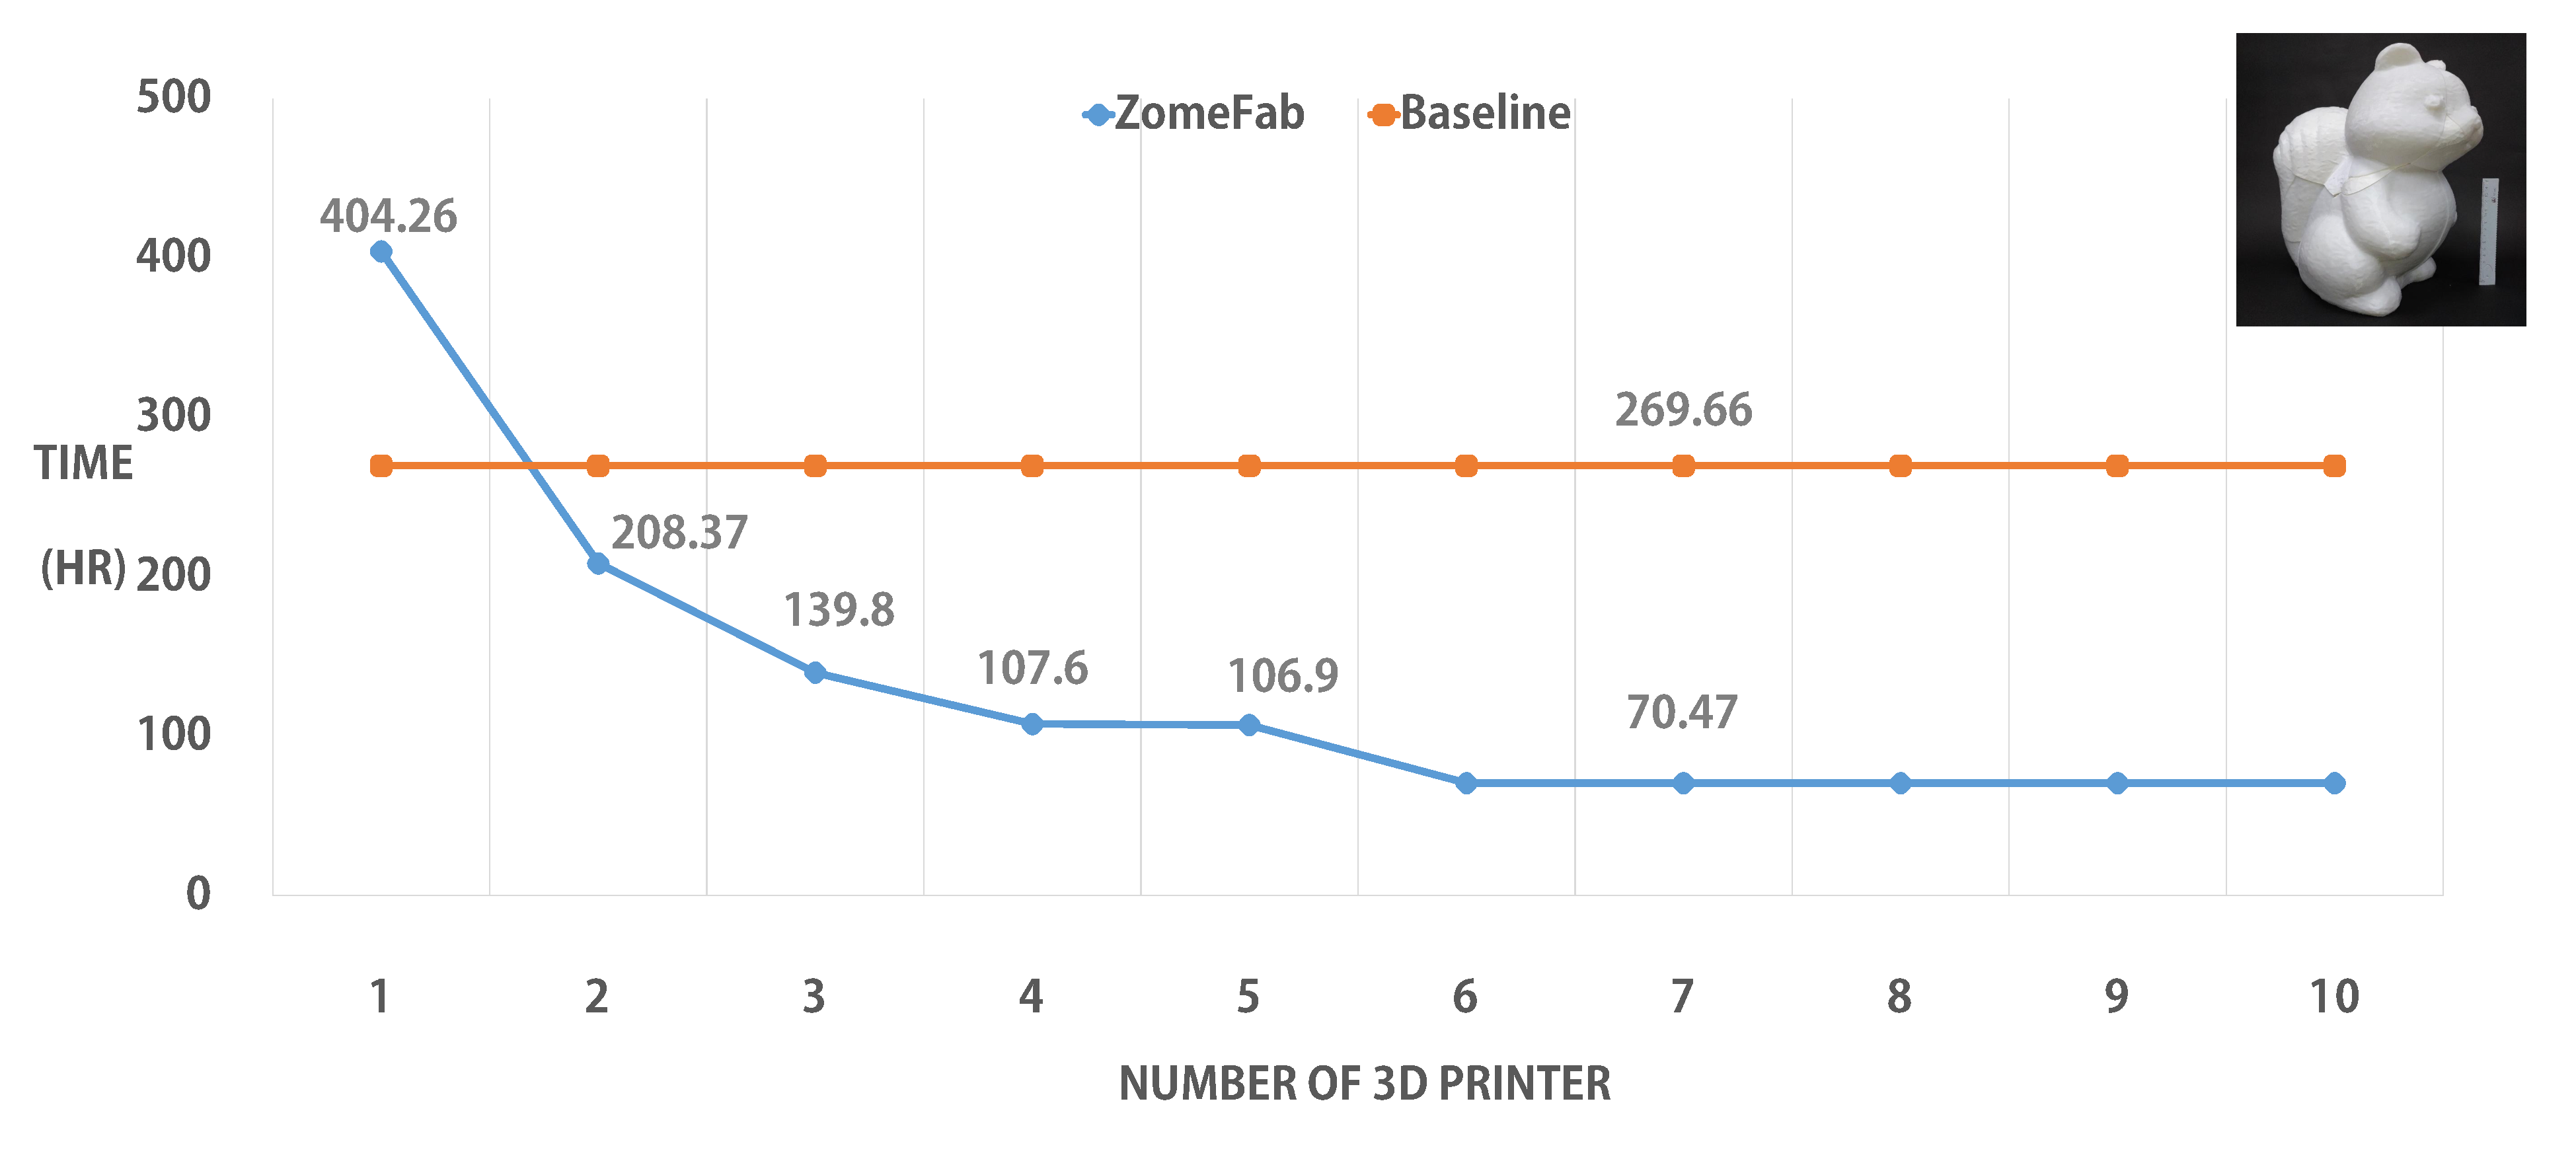
\includegraphics[width=1.0\linewidth]{figs/multi_printer.pdf} 
\caption{Printing time of Squirrel with different number of printers. If user use single 3D printer to print the result, our method's printing time will be more than baseline. The chart shows if the number of 3D printers are more than 2, the printing time will lower than baseline. If user has more than 6 3D printers, the printing time only has to wait the pieces which has the longest printing time.
}
\label{fig:multi_printer}
\end{figure*}

\begin{table*}[ht]
\centering
\resizebox{0.7\linewidth}{!} {
\begin{tabular}{|c|c|c|c|c|c|c|c|c|c|c|c|} \hline
\multirow{3}*{Mesh} & \multicolumn{10}{c|}{Zometool} & \multirow{3}*{Printing pieces}\\\cline{2-11} 
& \multicolumn{3}{c|}{Blue} & \multicolumn{3}{c|}{Red} & \multicolumn{3}{c|}{Yellow} & \multirow{2}*{Ball} & \\\cline{2-10} 
& S & M & L & S & M & L & S & M & L & & \\ \hline
Moai & 112 & 0 & 0 & 0 & 0 & 0 & 140 & 0 & 0 & 73 & 8 \\ \hline
Squirrel & 144 & 22 & 0 & 8 & 4 & 0 & 119 & 3 & 1 & 85 & 13 \\ \hline
Doraemon & 143 & 26 & 1 & 2 & 5 & 1 & 89 & 1 & 1 & 87 & 15 \\ \hline
Totoro & 95 & 0 & 0 & 0 & 0 & 0 & 137 & 0 & 0 & 60 & 18 \\ \hline
Iron Man & 93 & 0 & 0 & 0 & 0 & 0 & 124 & 0 & 0 & 57 & 10 \\ \hline
Owl & 115 & 0 & 0 & 0 & 0 & 0 & 159 & 0 & 0 & 70 & 15 \\ \hline
Pig & 61 & 12 & 0 & 10 & 8 & 0 & 53 & 6 & 0 & 47 & 10 \\ \hline
Slime & 132 & 0 & 0 & 0 & 0 & 0 & 182 & 0 & 0 & 80 & 14 \\ \hline
Lion & 78 & 0 & 0 & 0 & 0 & 0 & 101 & 0 & 0 & 50 & 8 \\ \hline
Bunny & 215 & 0 & 0 & 0 & 0 & 0 & 266 & 0 & 0 & 126 & 10 \\ \hline
\end{tabular}
}
\caption{Material usage for each result. Including Zometool and printing pieces.}
\label{tab:result_Zometool}
\end{table*}

% \begin{table*}[ht]
% \centering
% \resizebox{0.95\linewidth}{!} {
% \begin{tabular}{c} 
% 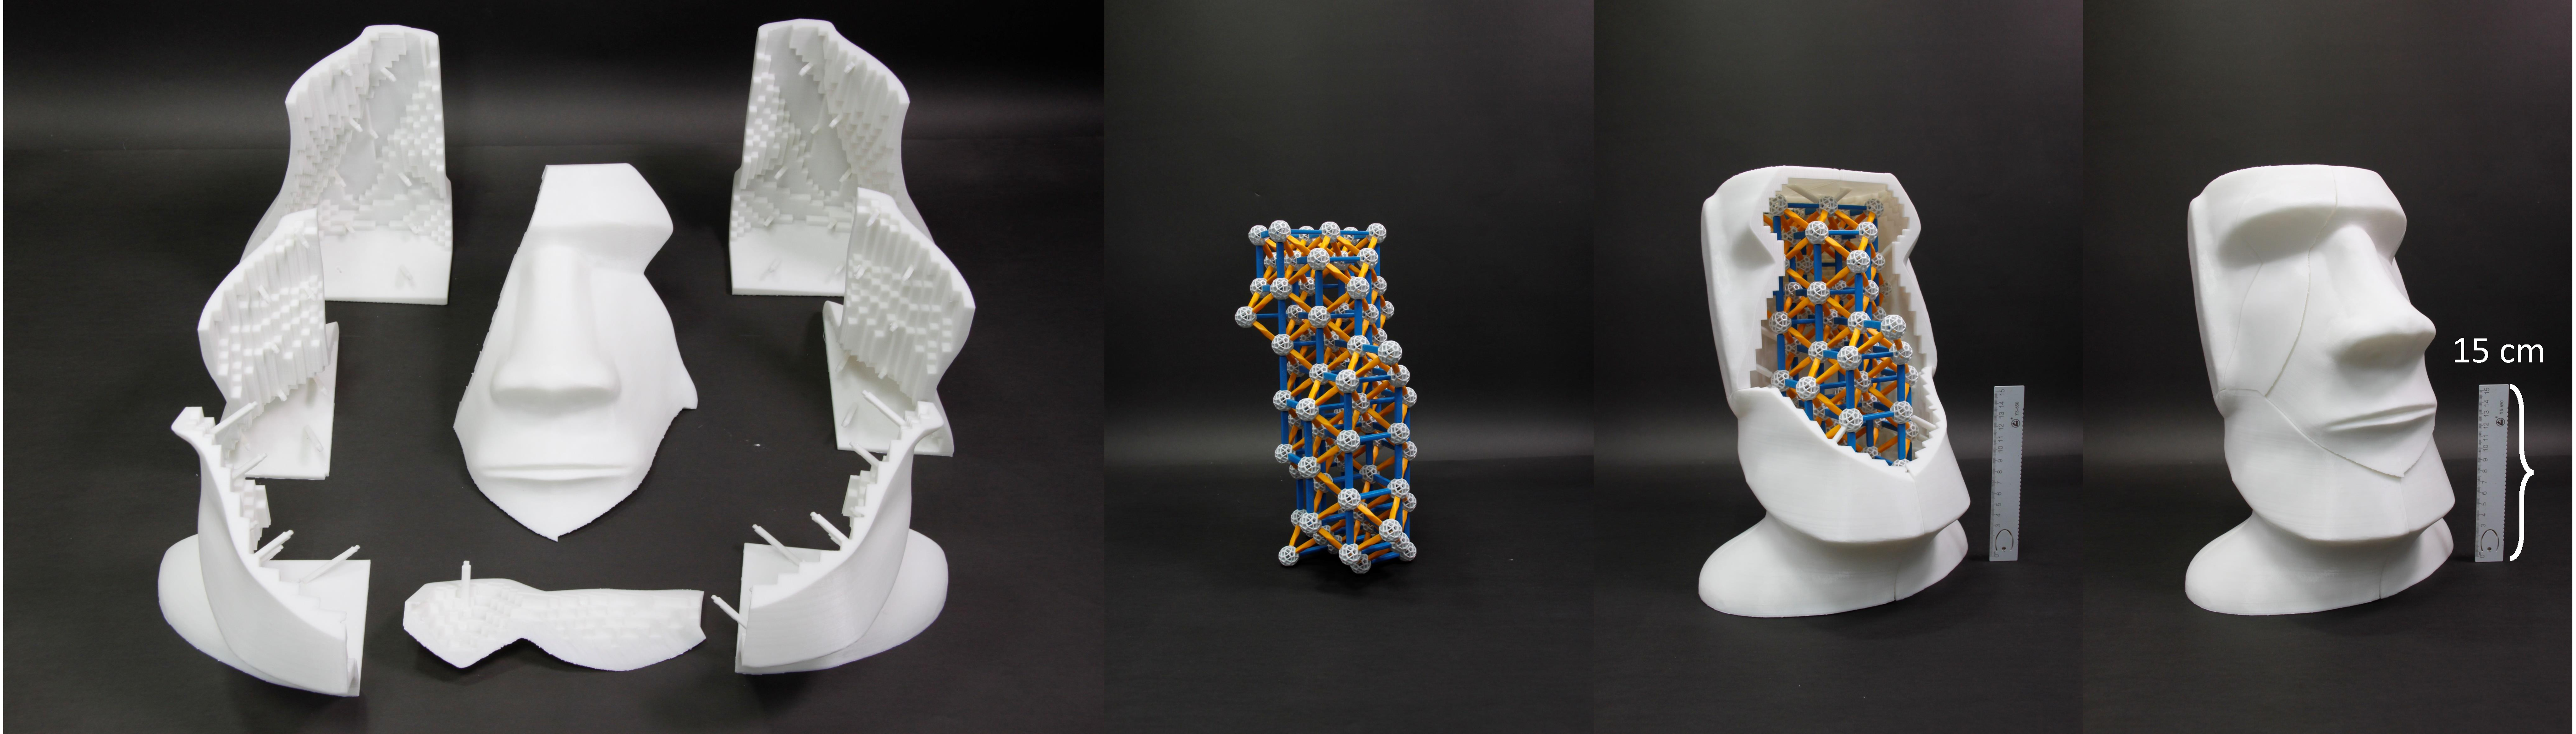
\includegraphics{figs/MOAI_real.pdf} \\
% \includegraphics{figs/Squirrel_real.pdf}\\
% 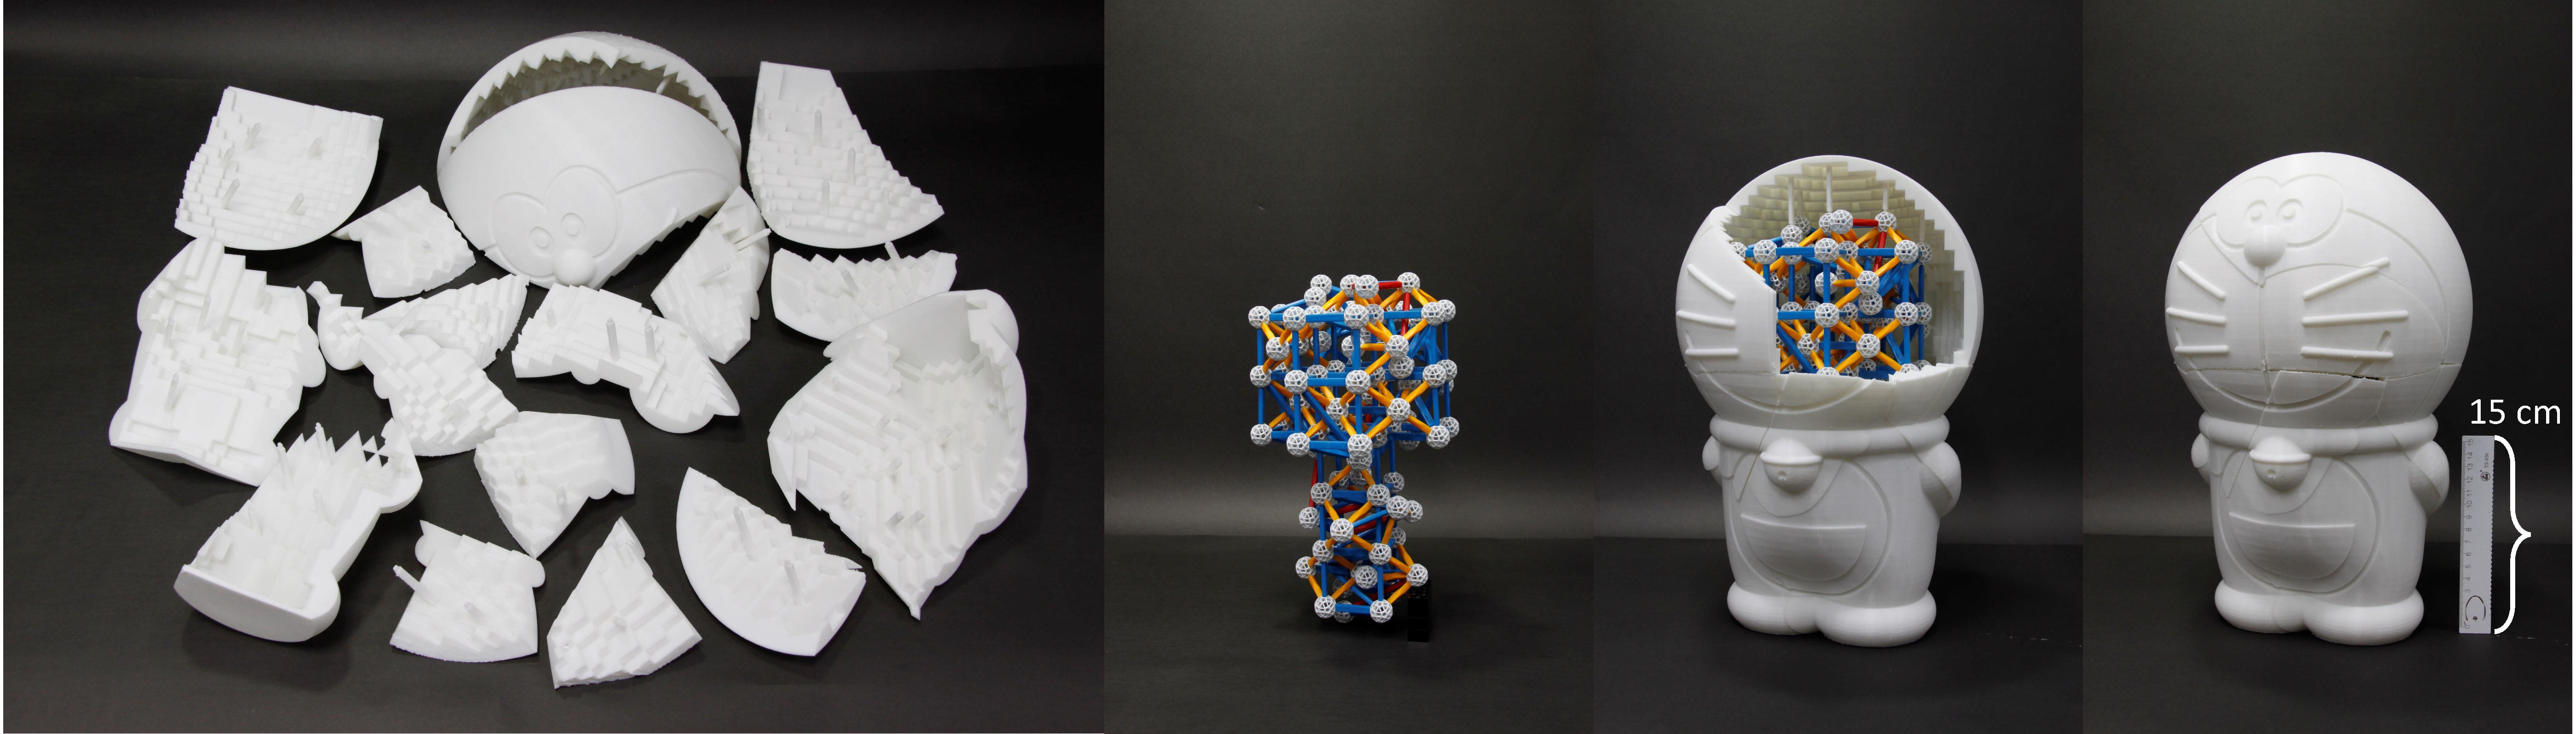
\includegraphics{figs/doraemon_real.pdf}\\
% 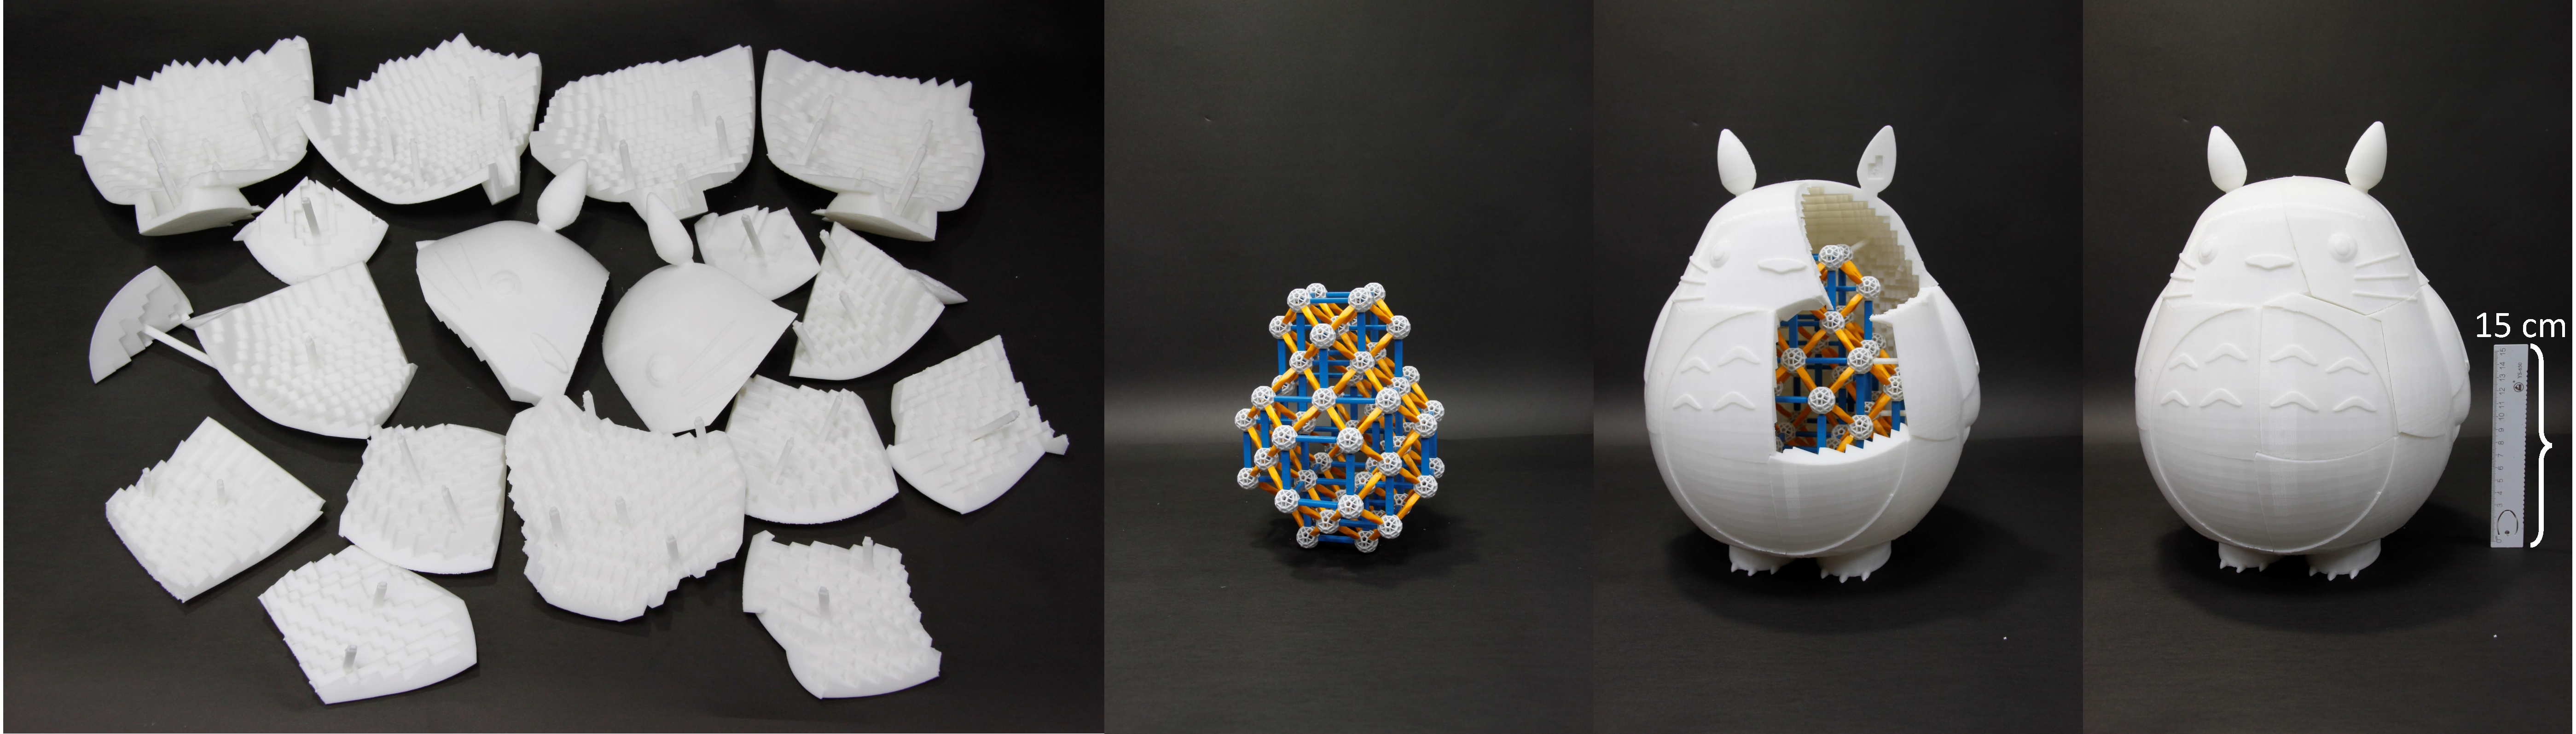
\includegraphics{figs/totoro_real.pdf}\\
% 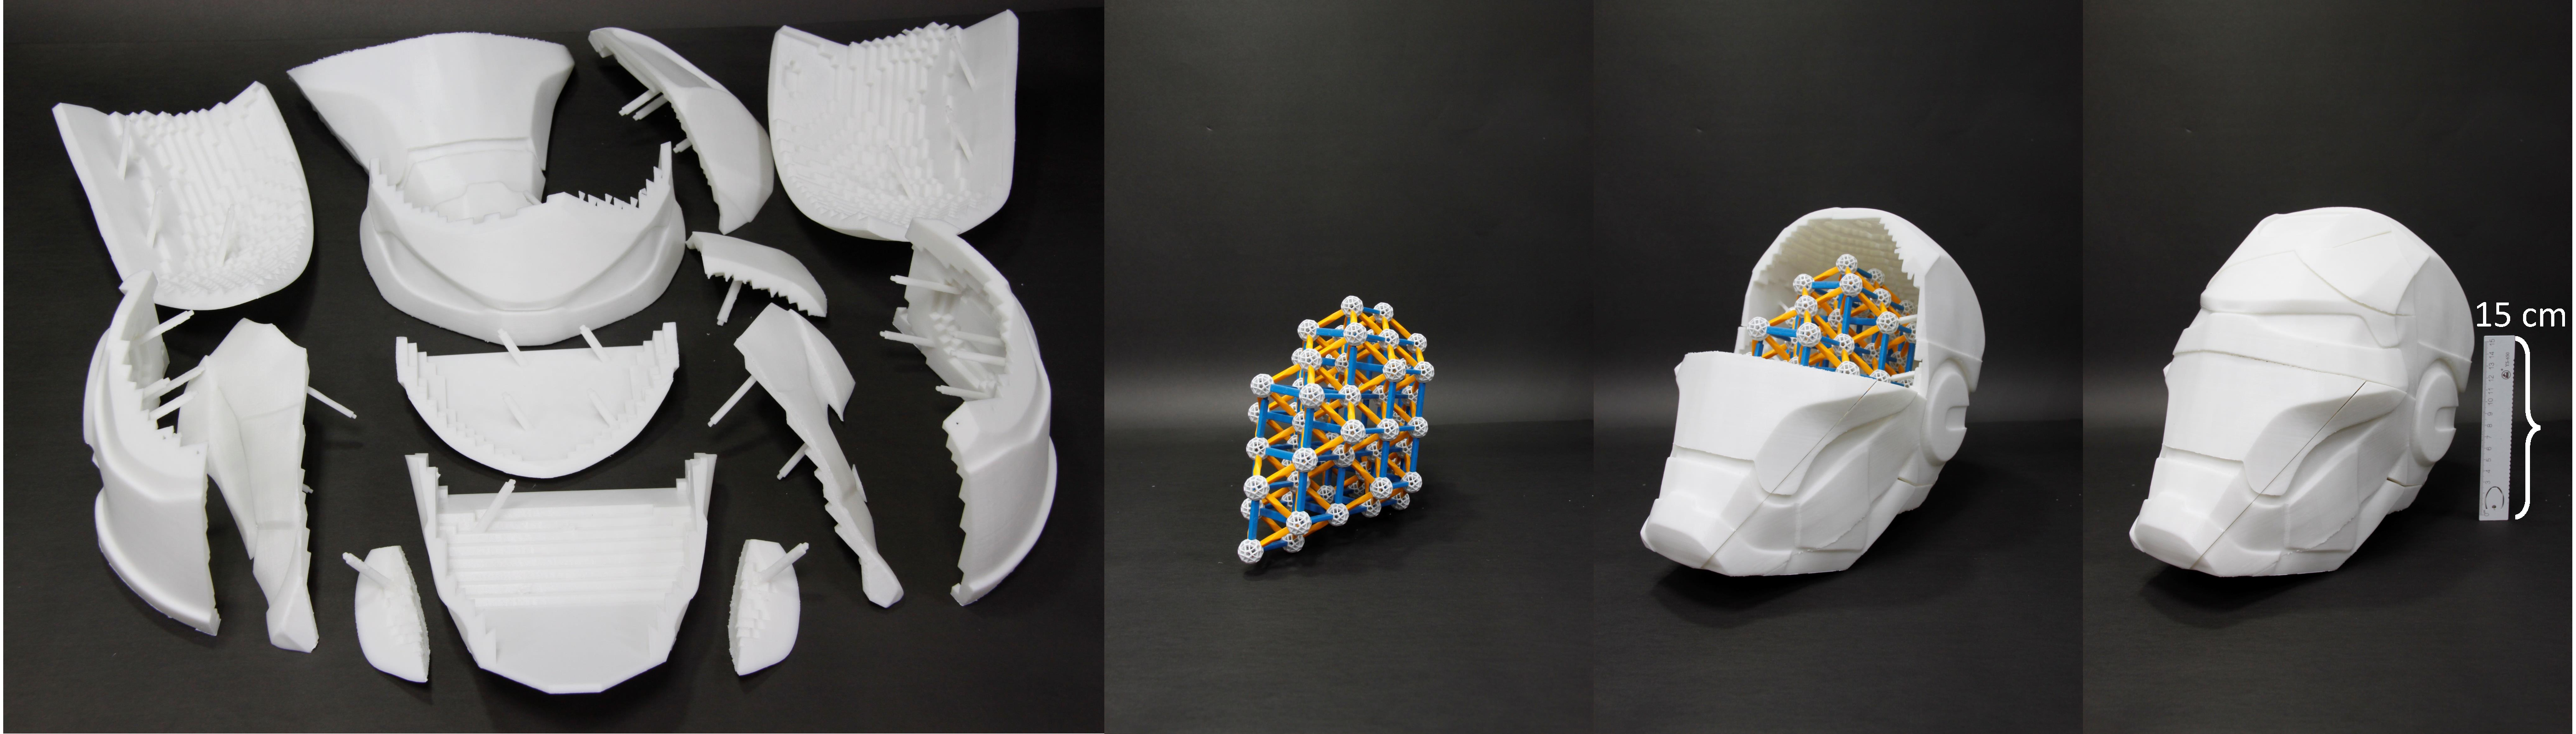
\includegraphics{figs/iron_real.pdf}\\
% \end{tabular}
% }
% \caption{}
% \label{tab:result_ZomeFab_real}
% \end{table*}

\begin{table*}[ht]
\centering
\resizebox{0.965\linewidth}{!} {
\begin{tabular}{c} 
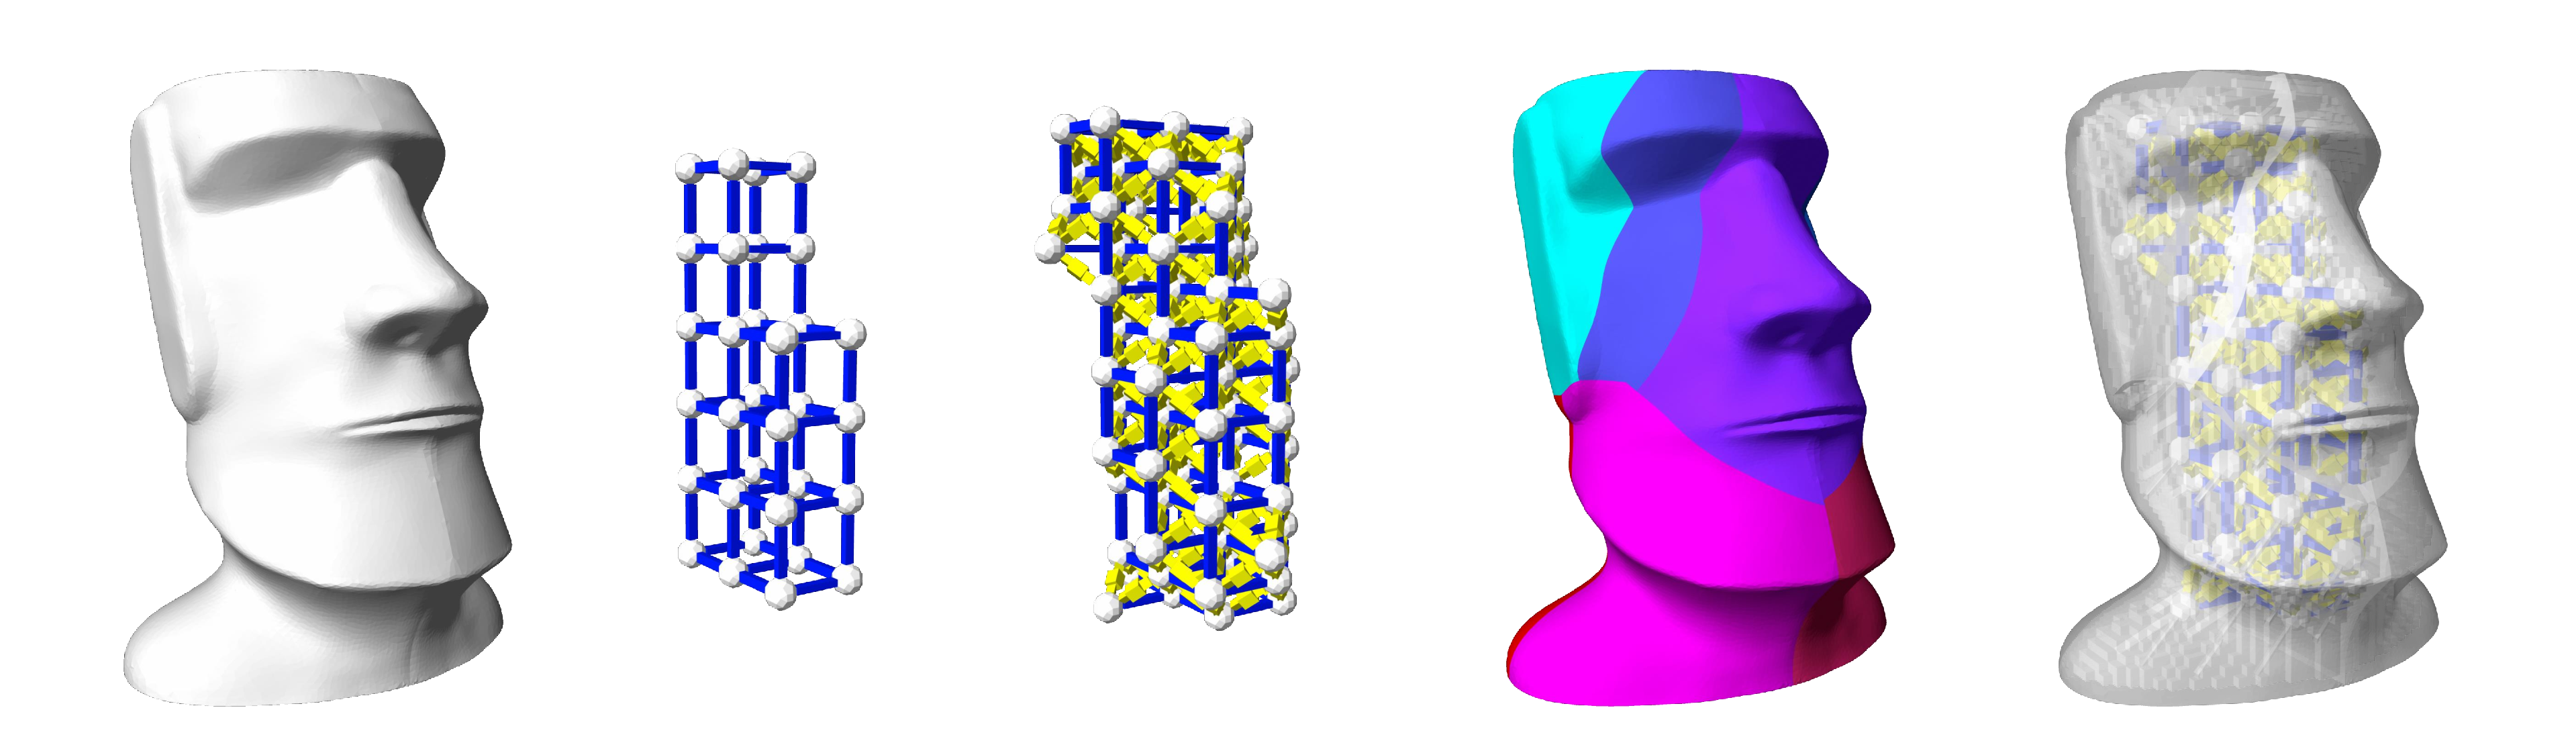
\includegraphics{figs/MOAI.pdf} \\
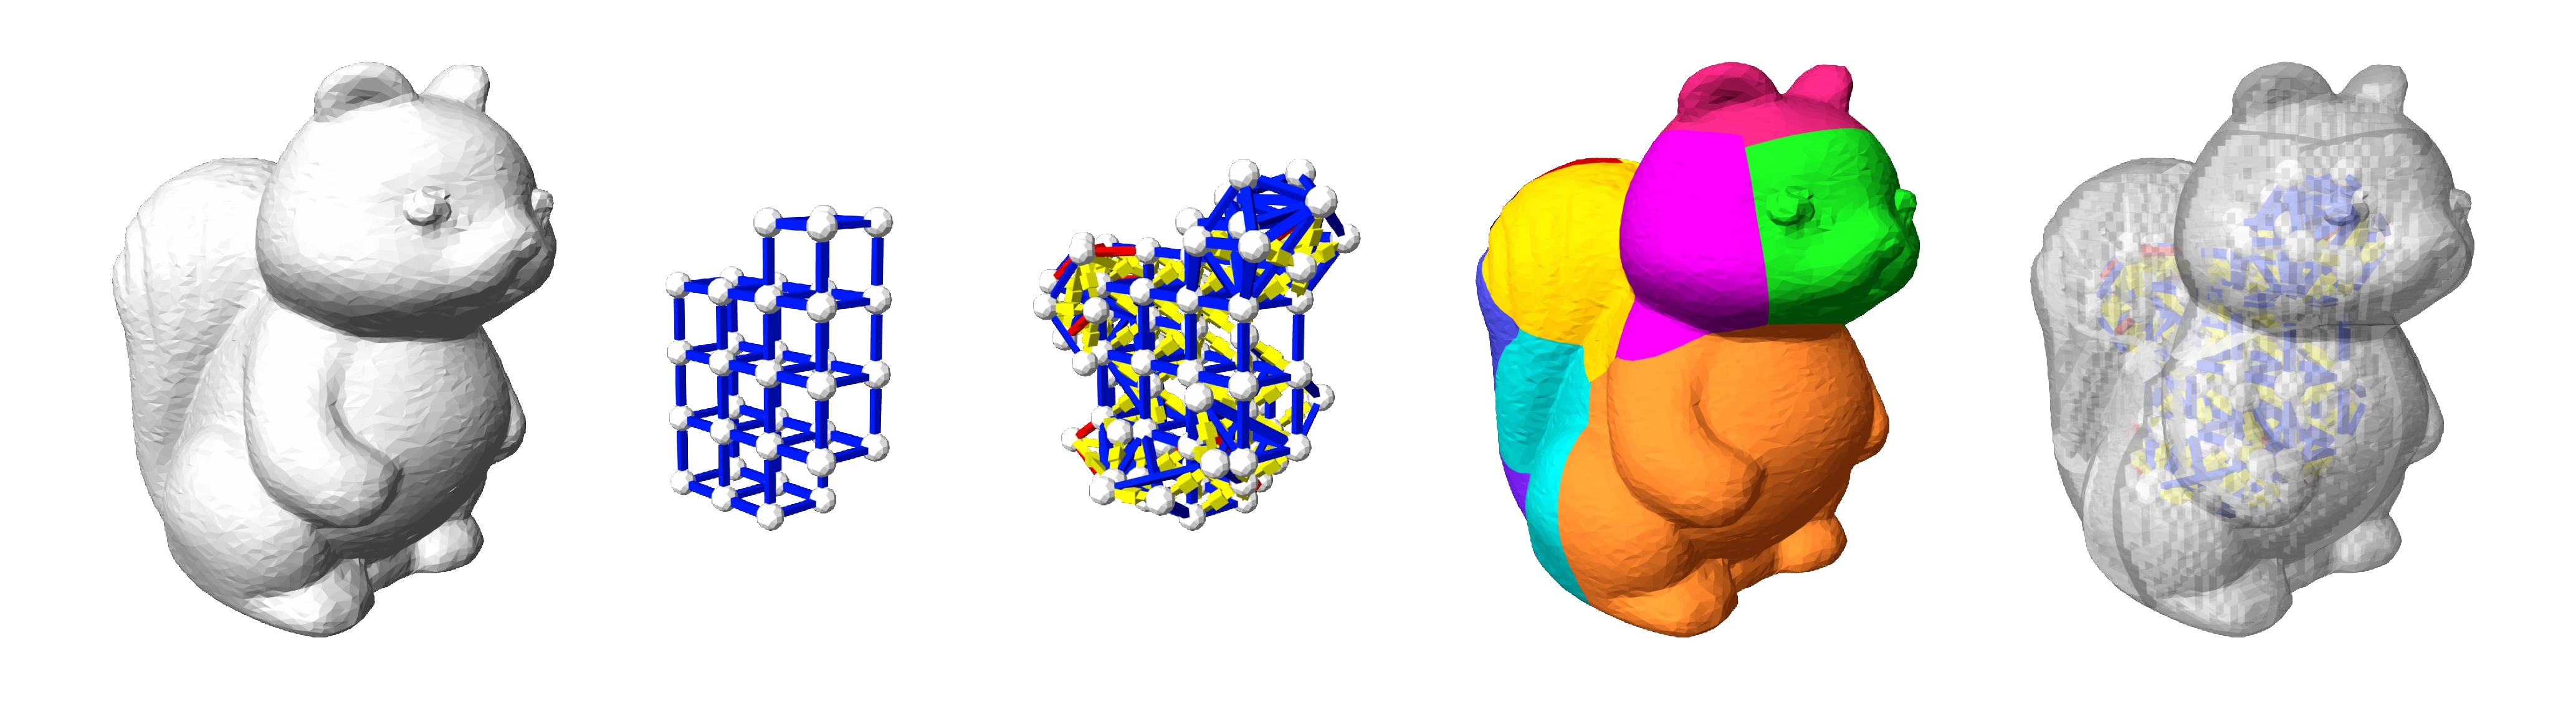
\includegraphics{figs/Squirrel.pdf}\\
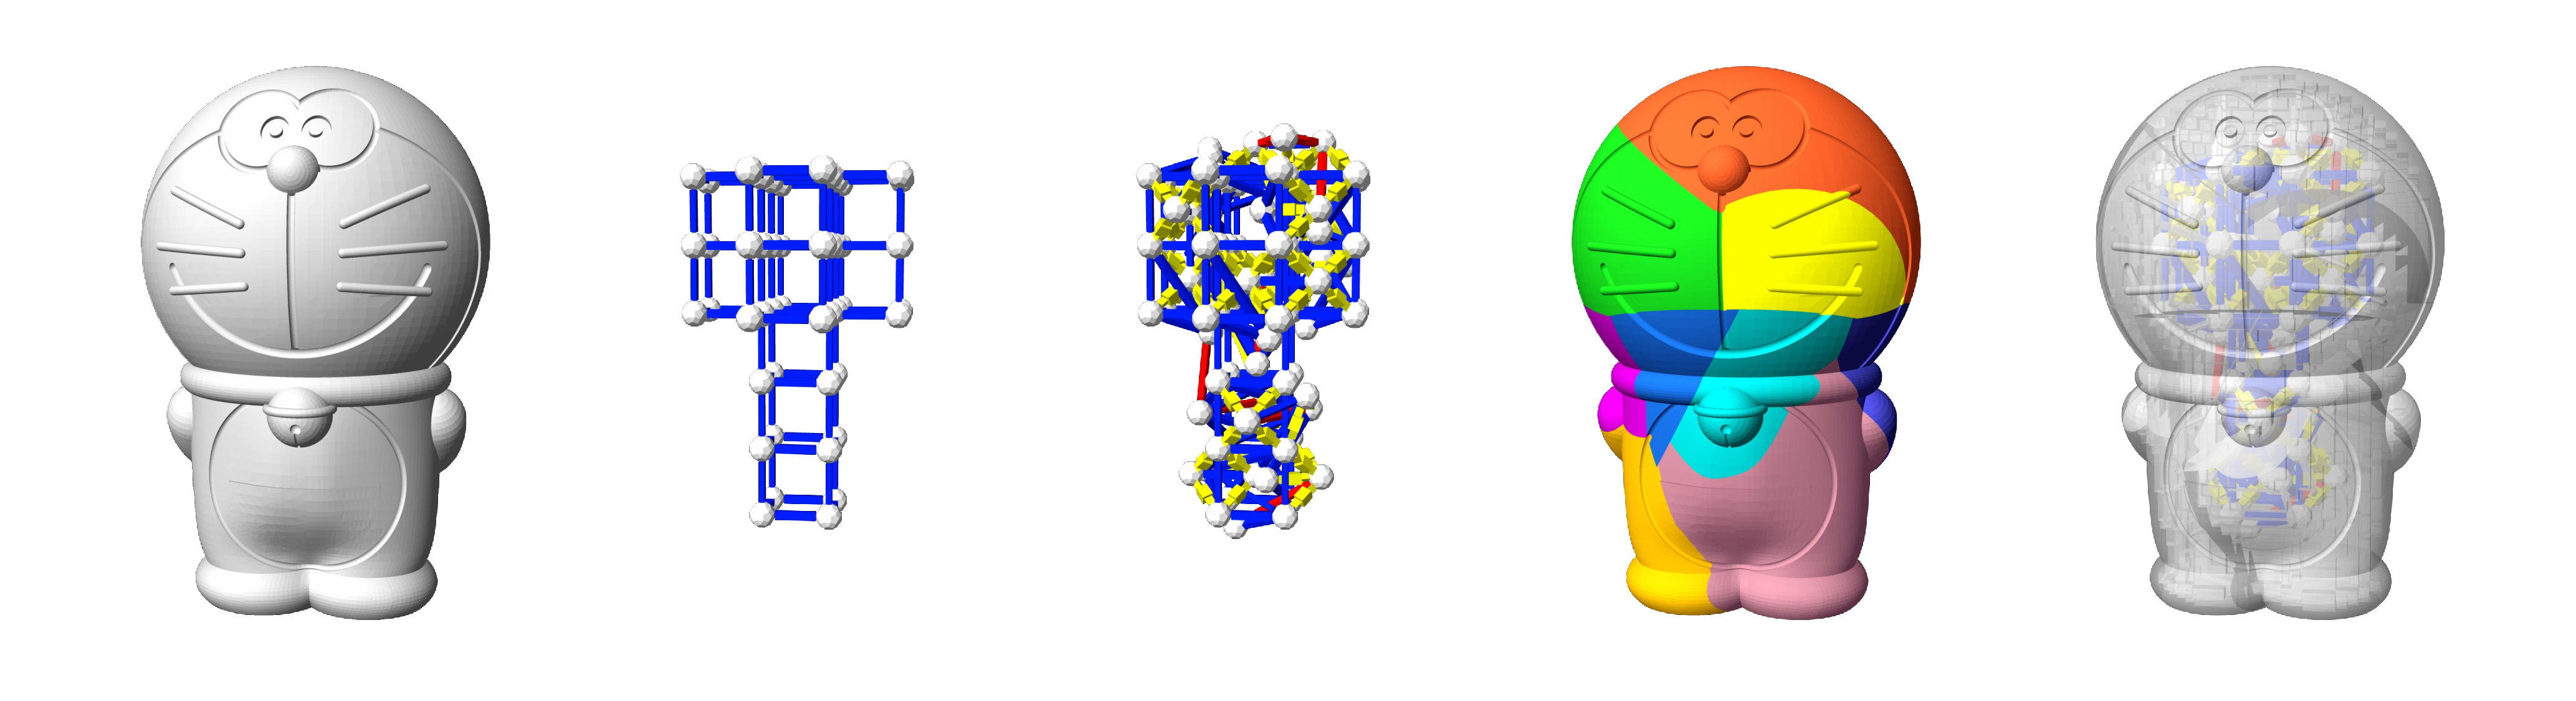
\includegraphics{figs/doraemon.pdf} \\
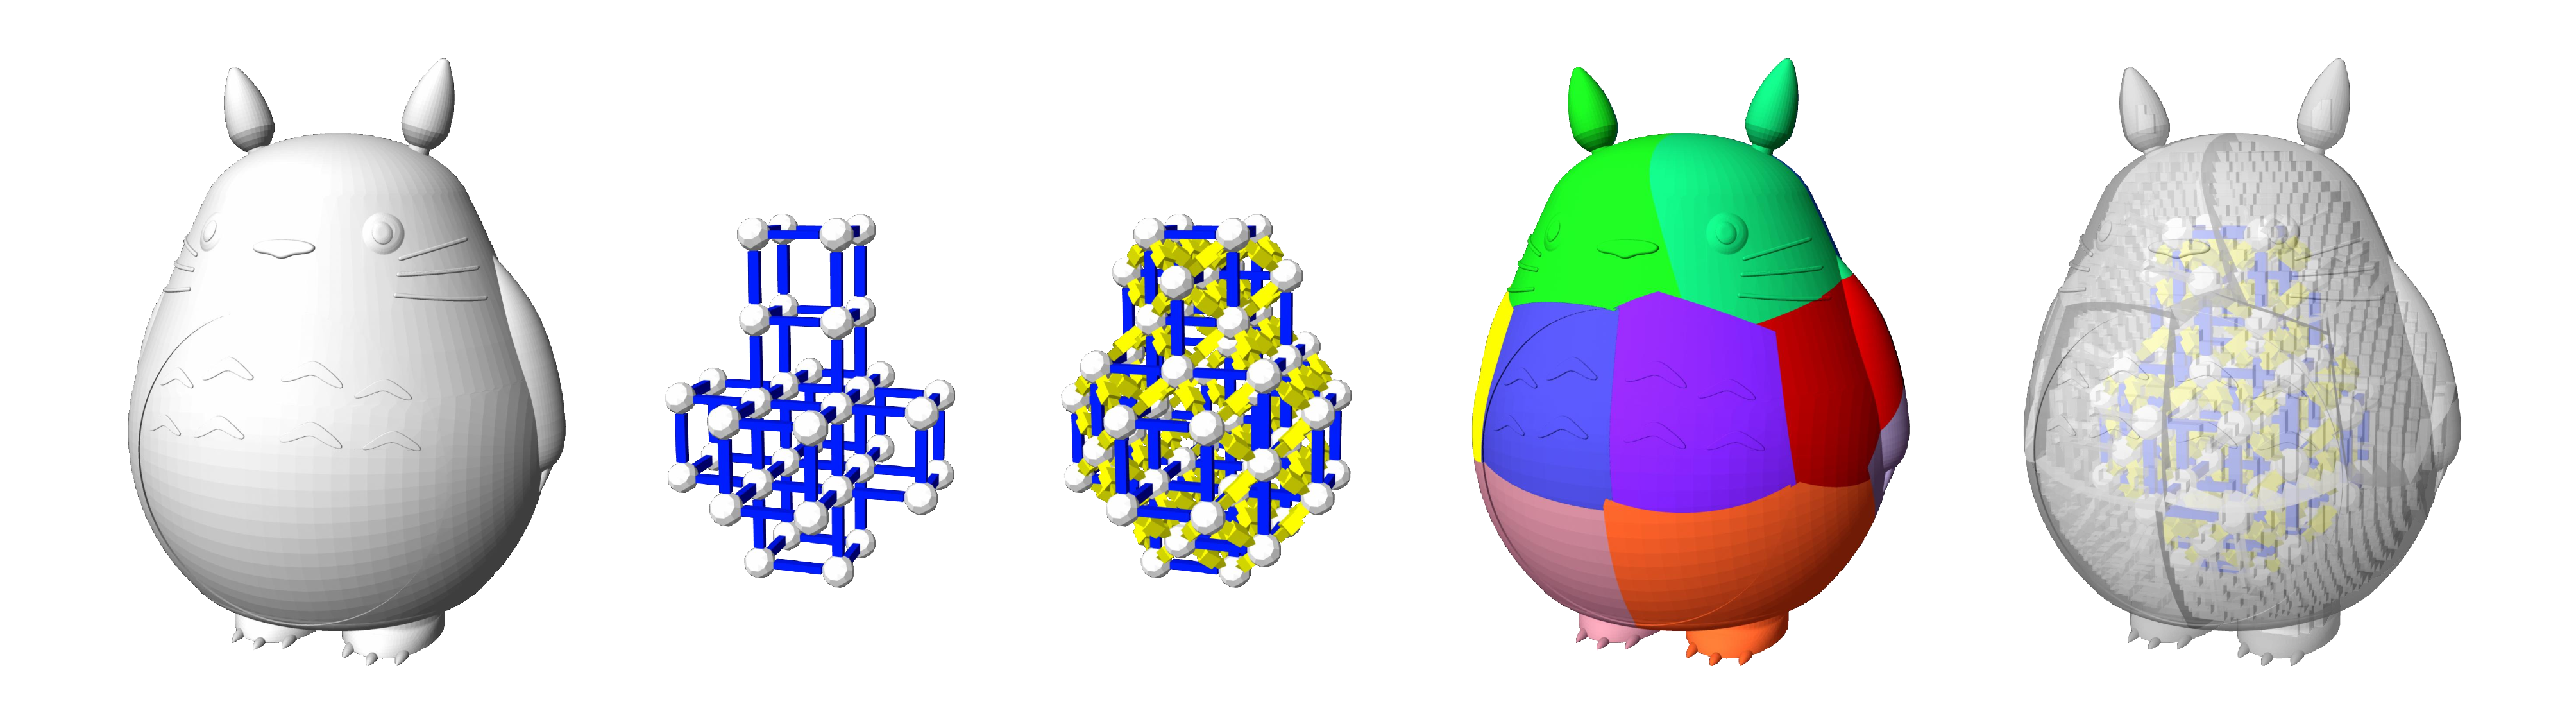
\includegraphics{figs/totoro.pdf}\\
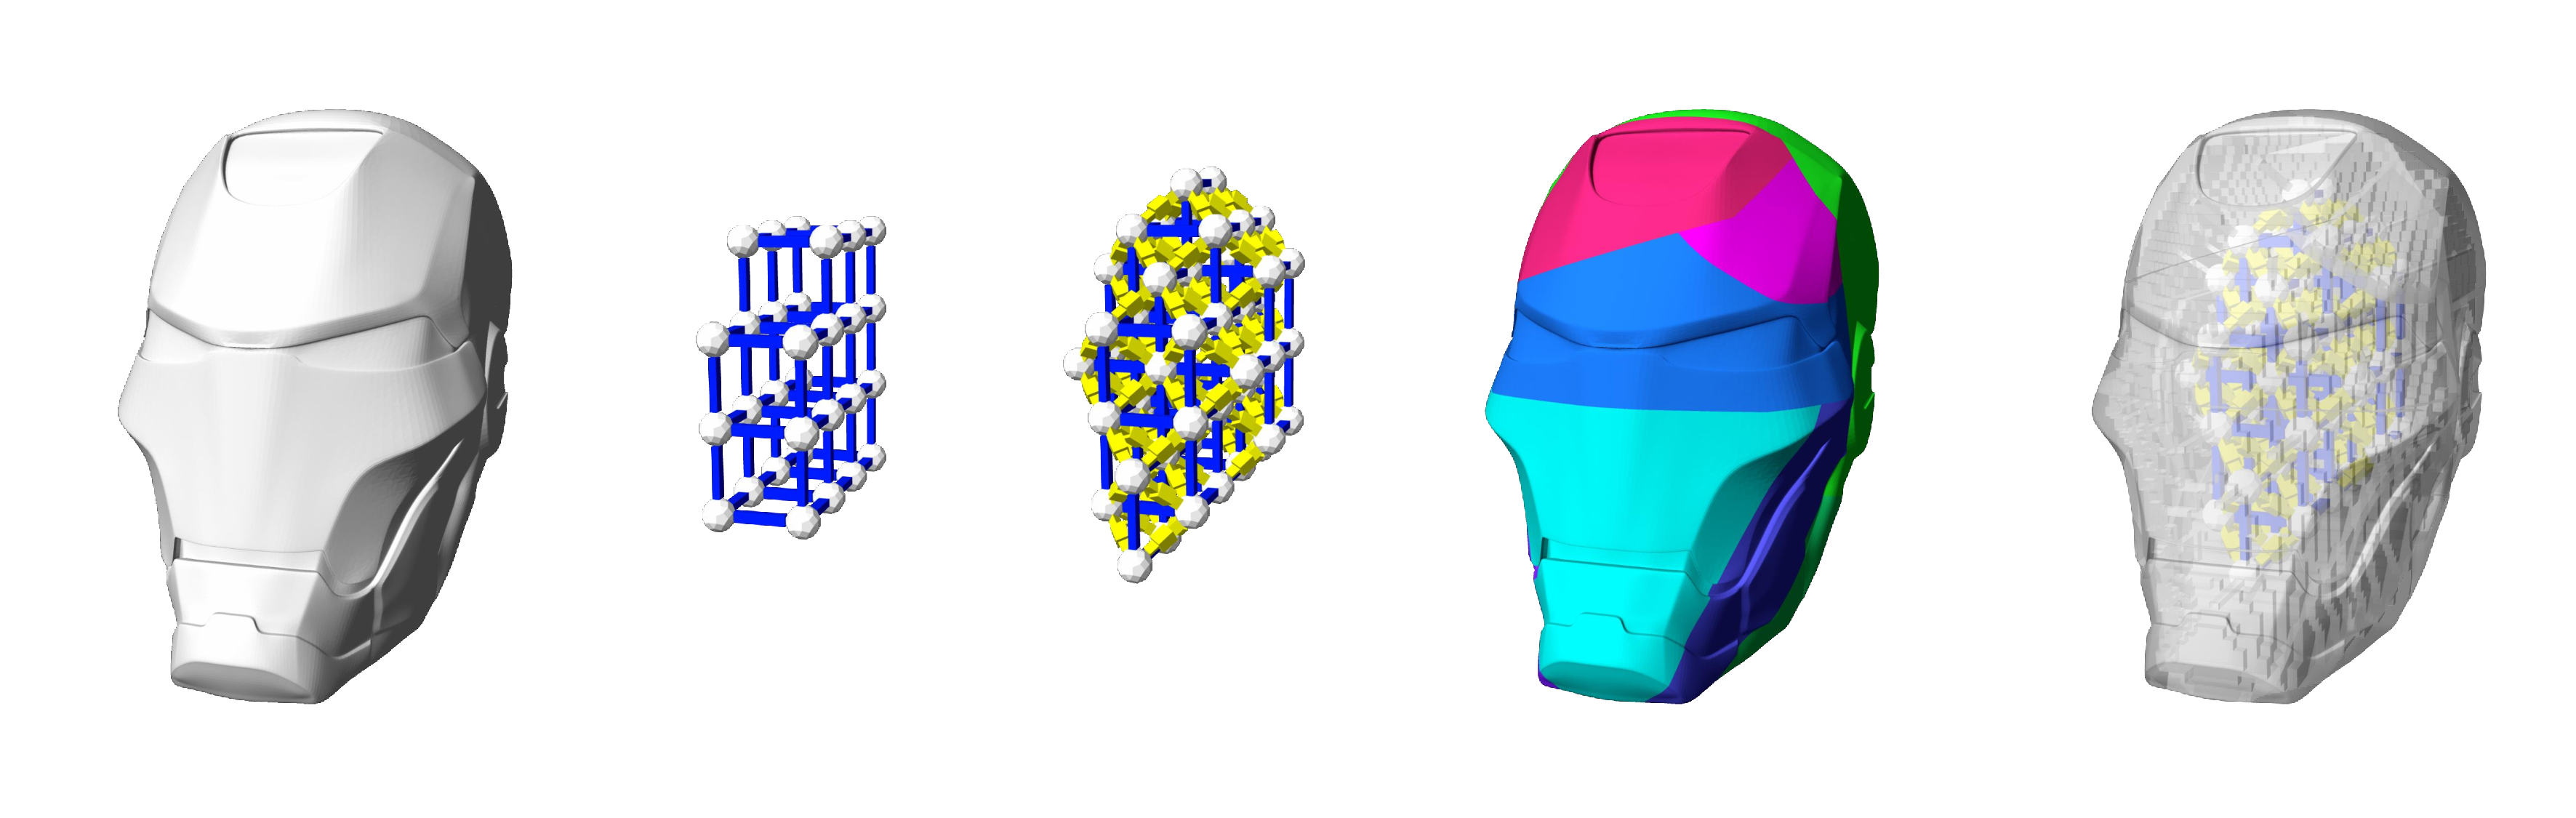
\includegraphics{figs/iron.pdf}\\
\end{tabular}
}
\caption{}
\label{tab:result_ZomeFab_file_1}
\end{table*}

\begin{table*}[ht]
\centering
\resizebox{1.\linewidth}{!} {
\begin{tabular}{c} 
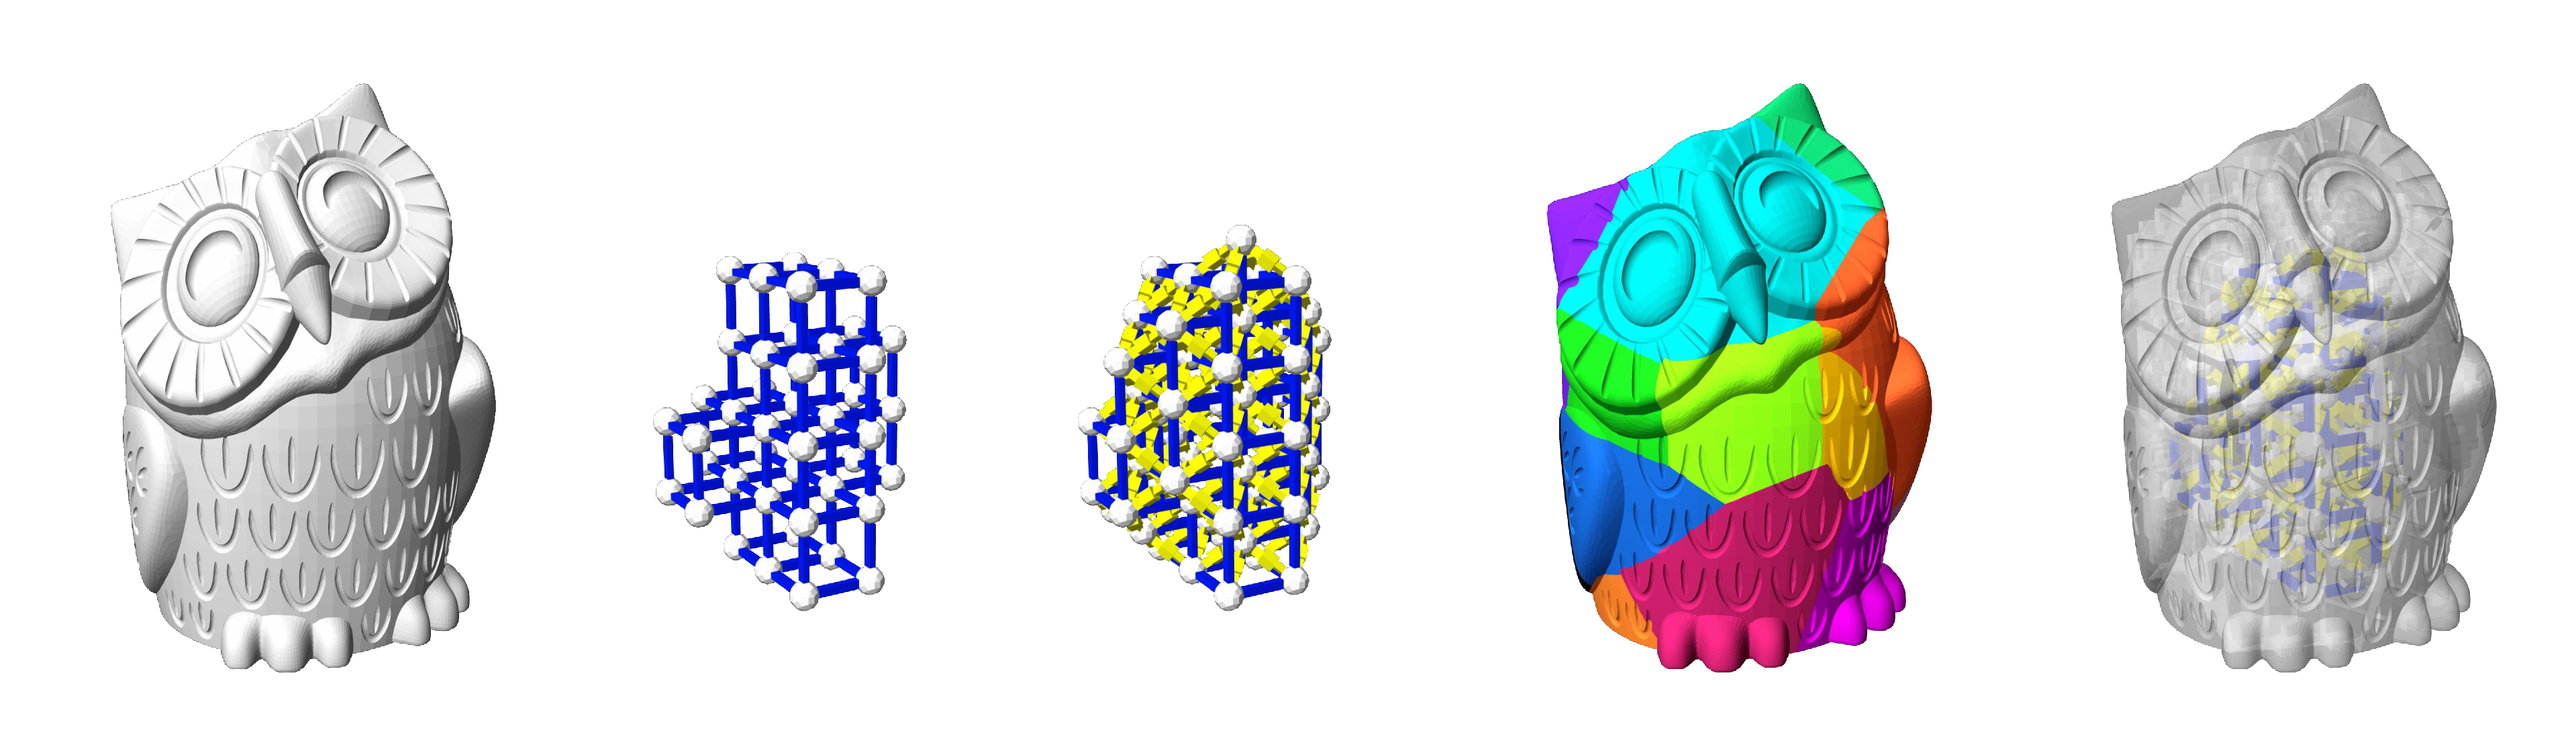
\includegraphics{figs/owl.pdf}\\
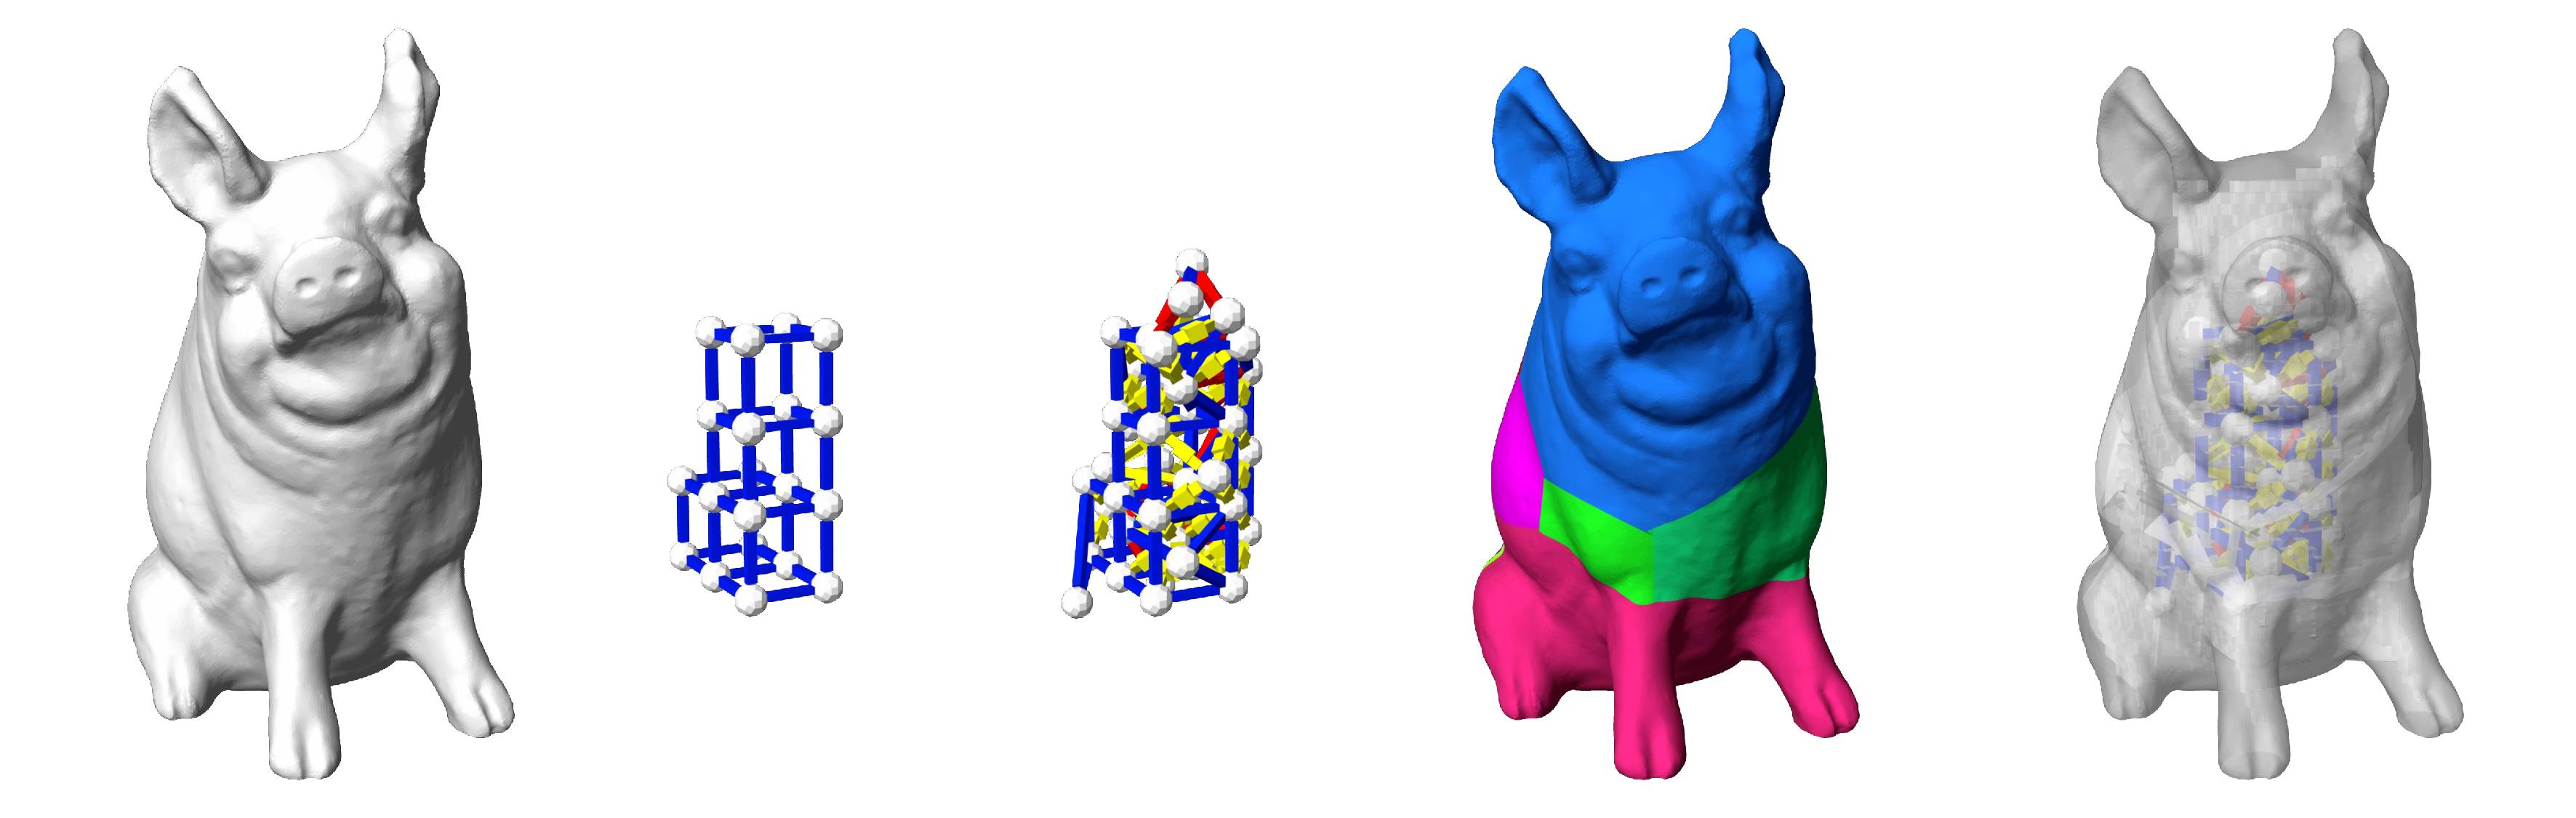
\includegraphics{figs/pig.pdf} \\
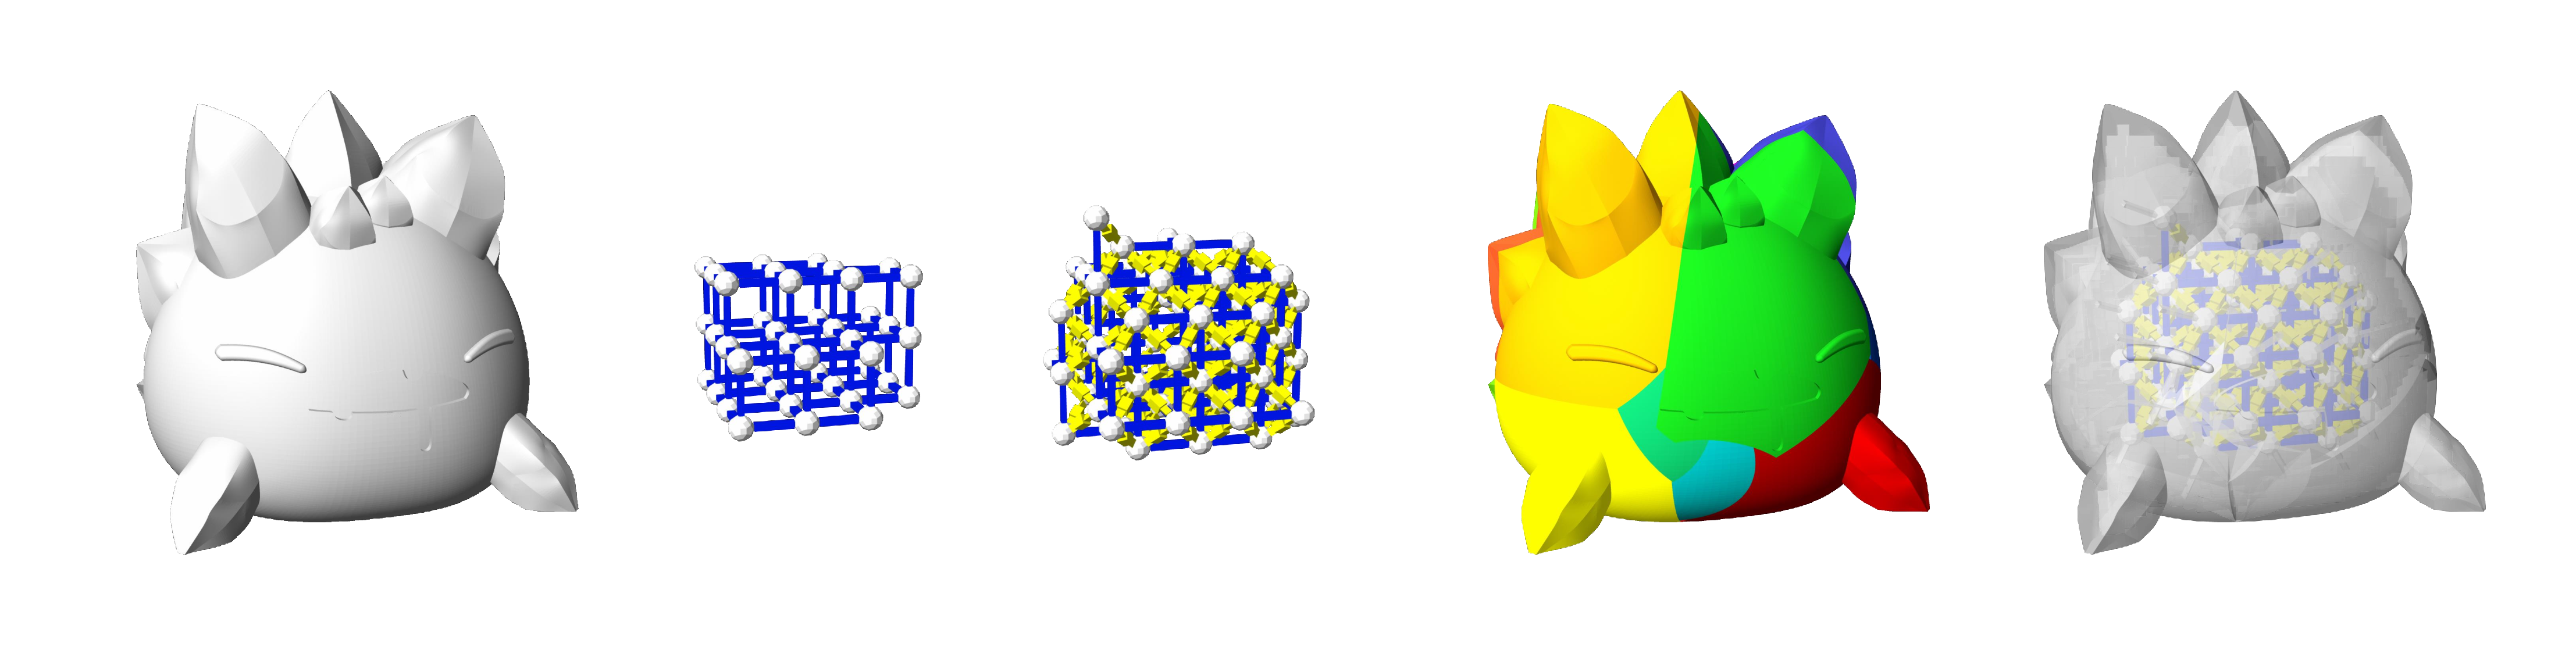
\includegraphics{figs/slime_high.pdf}\\
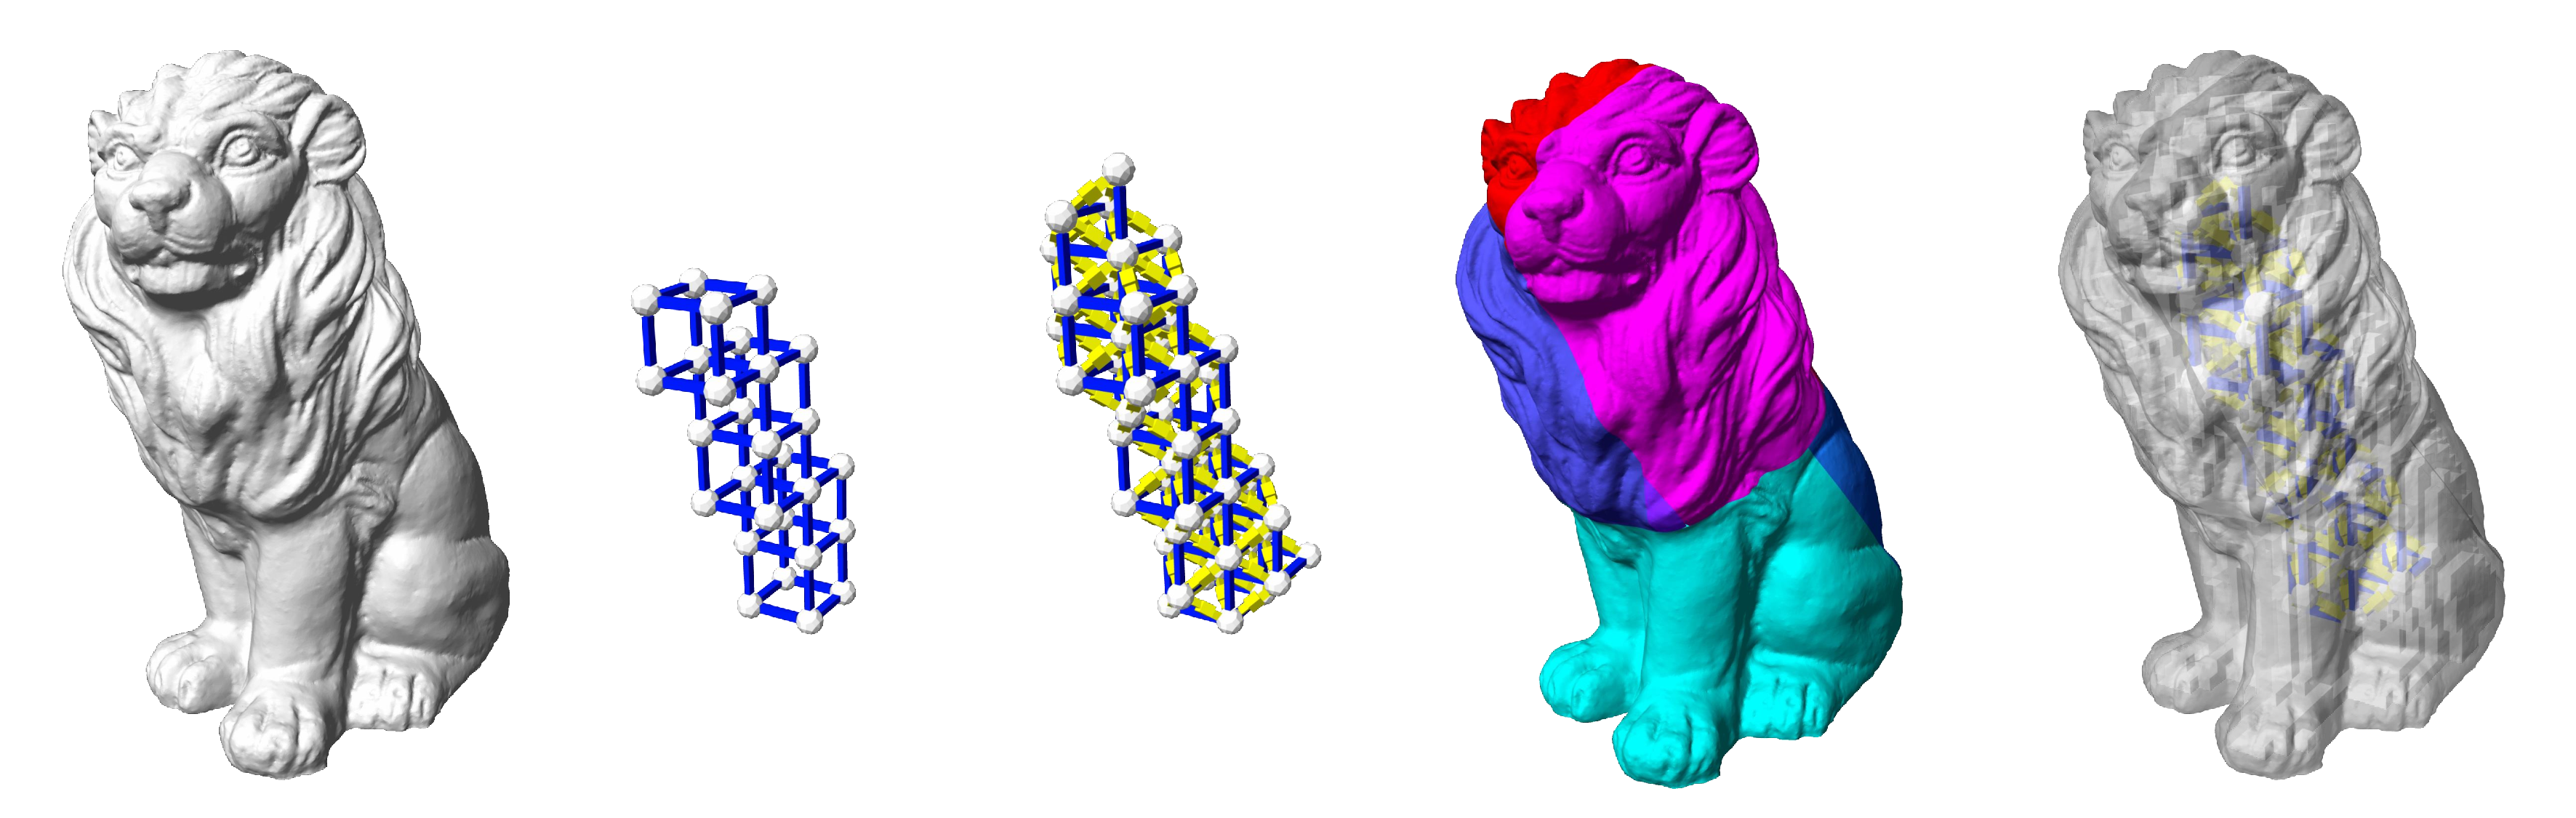
\includegraphics{figs/lion.pdf}\\
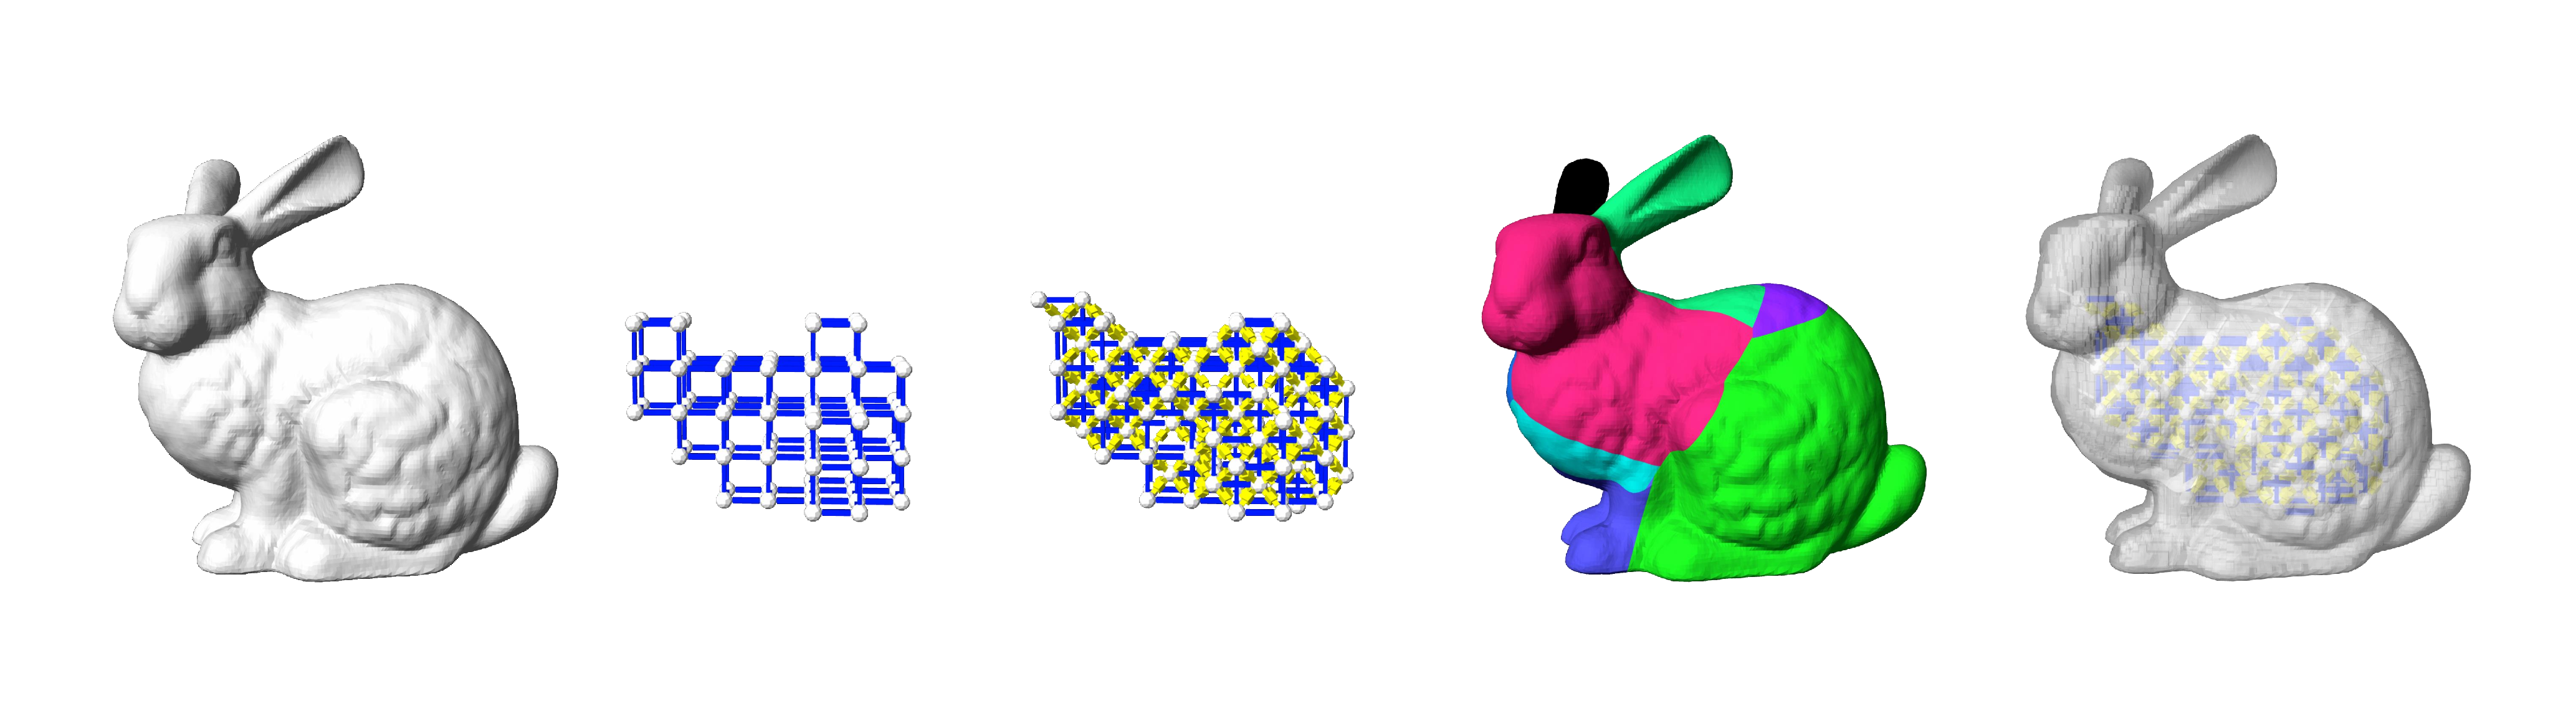
\includegraphics{figs/bunny_150.pdf}\\
\end{tabular}
}
\caption{}
\label{tab:result_ZomeFab_file_2}
\end{table*}

%\begin{figure*}[ht]
%\centering
%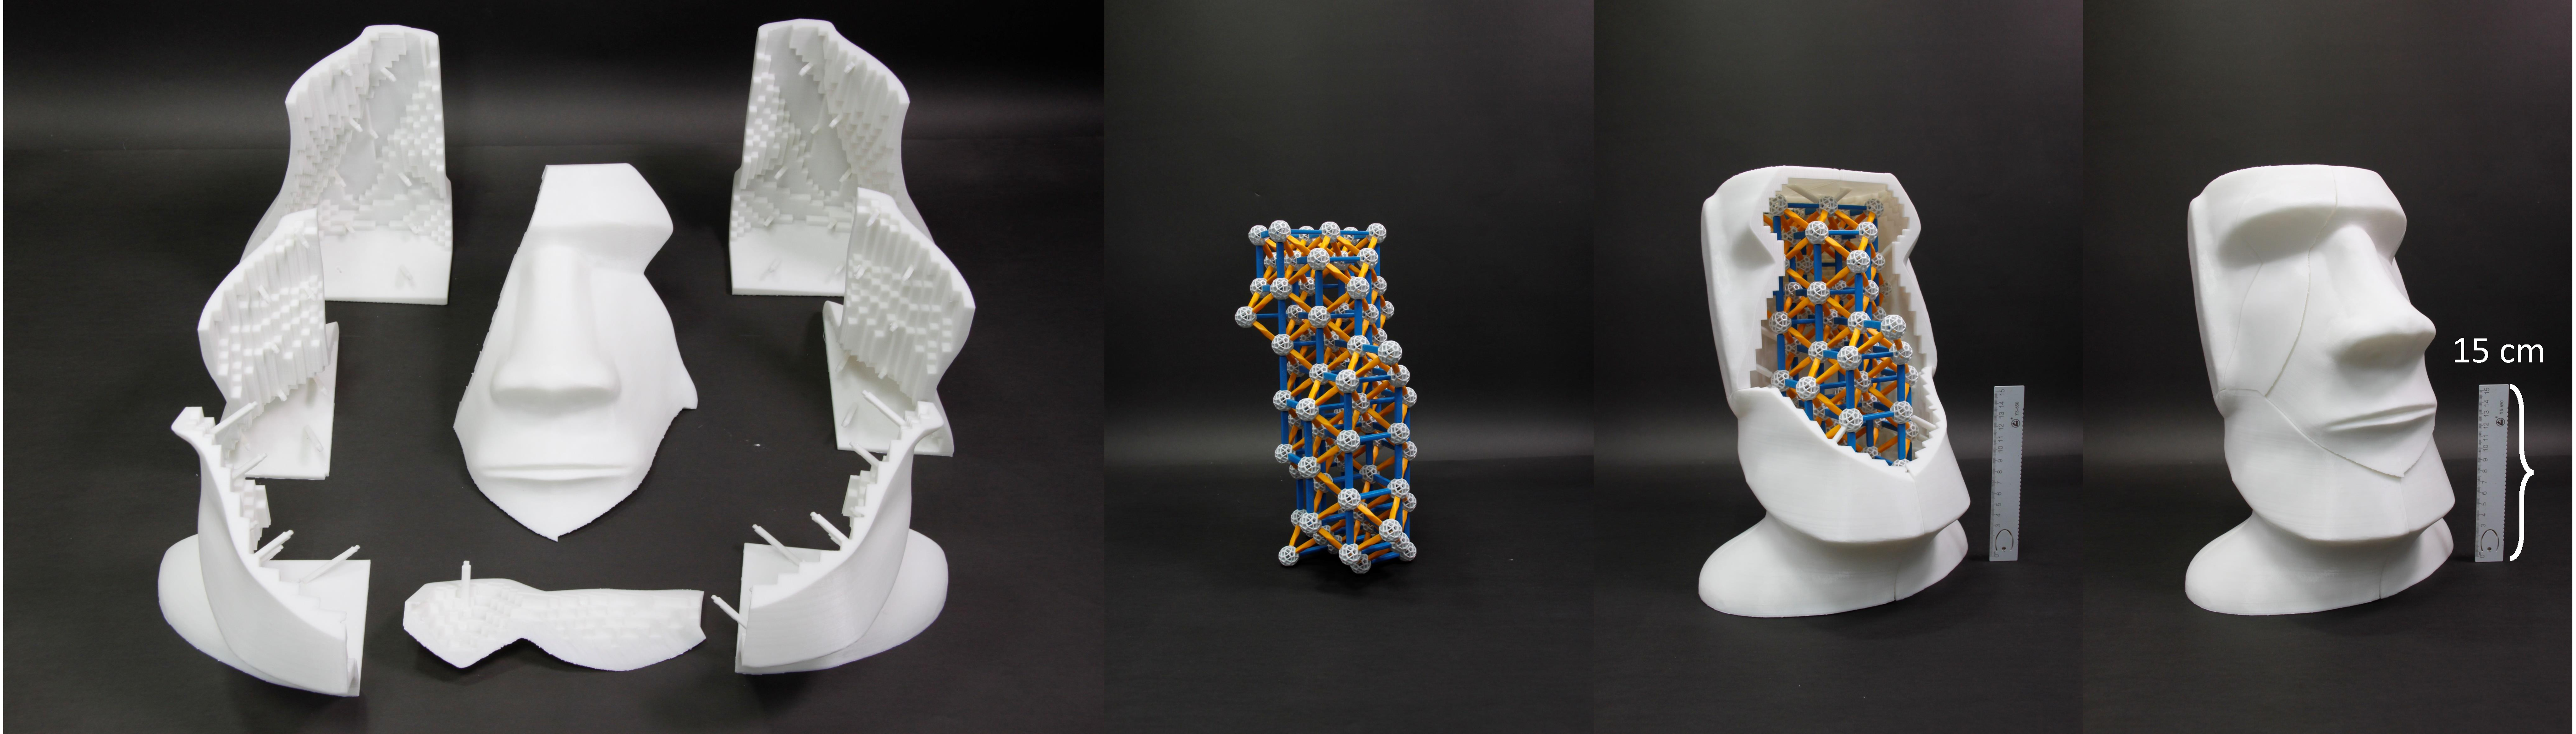
\includegraphics[width=1.0\linewidth]{figs/MOAI_real.pdf}
%\caption{Result fabricated and assembly : Moai}
%\label{fig:result-assembly_Moai_real}
%\end{figure*}

%\begin{figure*}[ht]
%\centering
%\includegraphics[width=1.0\linewidth]{figs/Squirrel_real.pdf} 
%\caption{Result fabricated and assembly : Squirrel}
%\label{fig:result-assembly_Squirrel_real}
%\end{figure*}

%\begin{figure*}[ht]
%\centering
%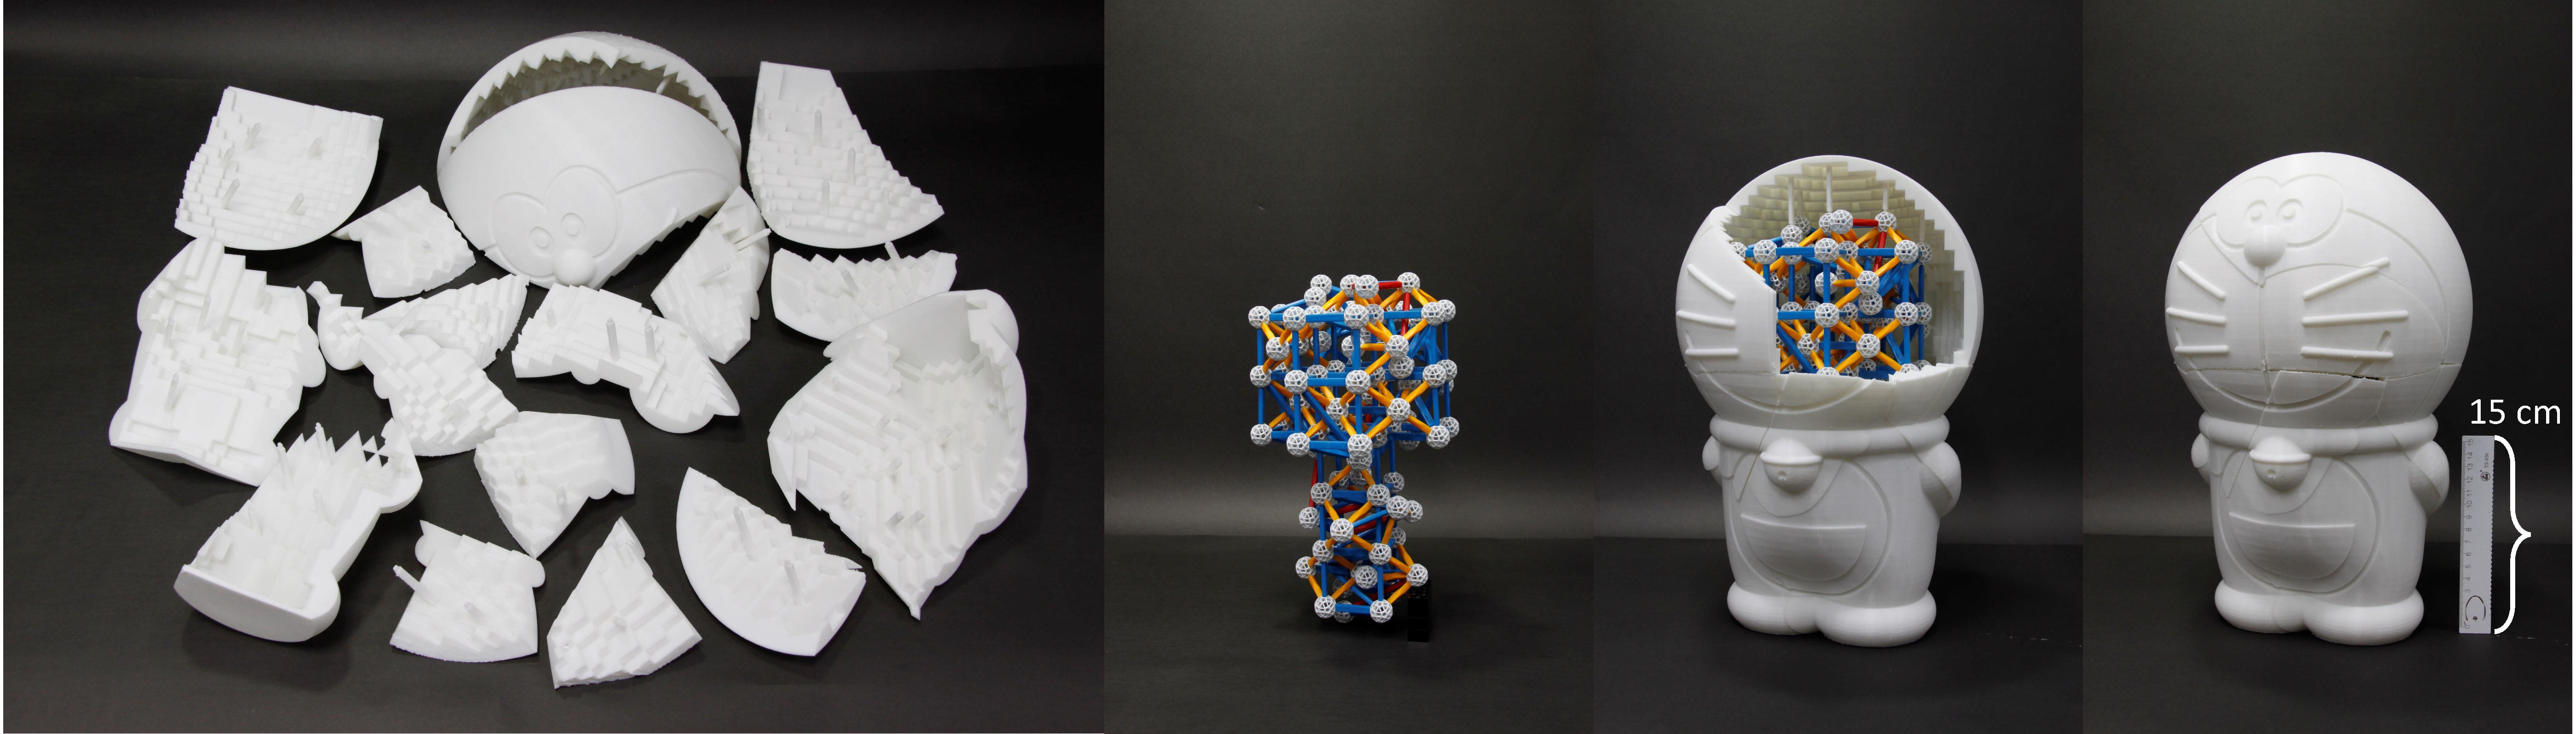
\includegraphics[width=1.0\linewidth]{figs/doraemon_real.pdf} 
%\caption{Result fabricated and assembly : Doraemon}
%\label{fig:result-assembly_doraemon_real}
%\end{figure*}

%\begin{figure*}[ht]
%\centering
%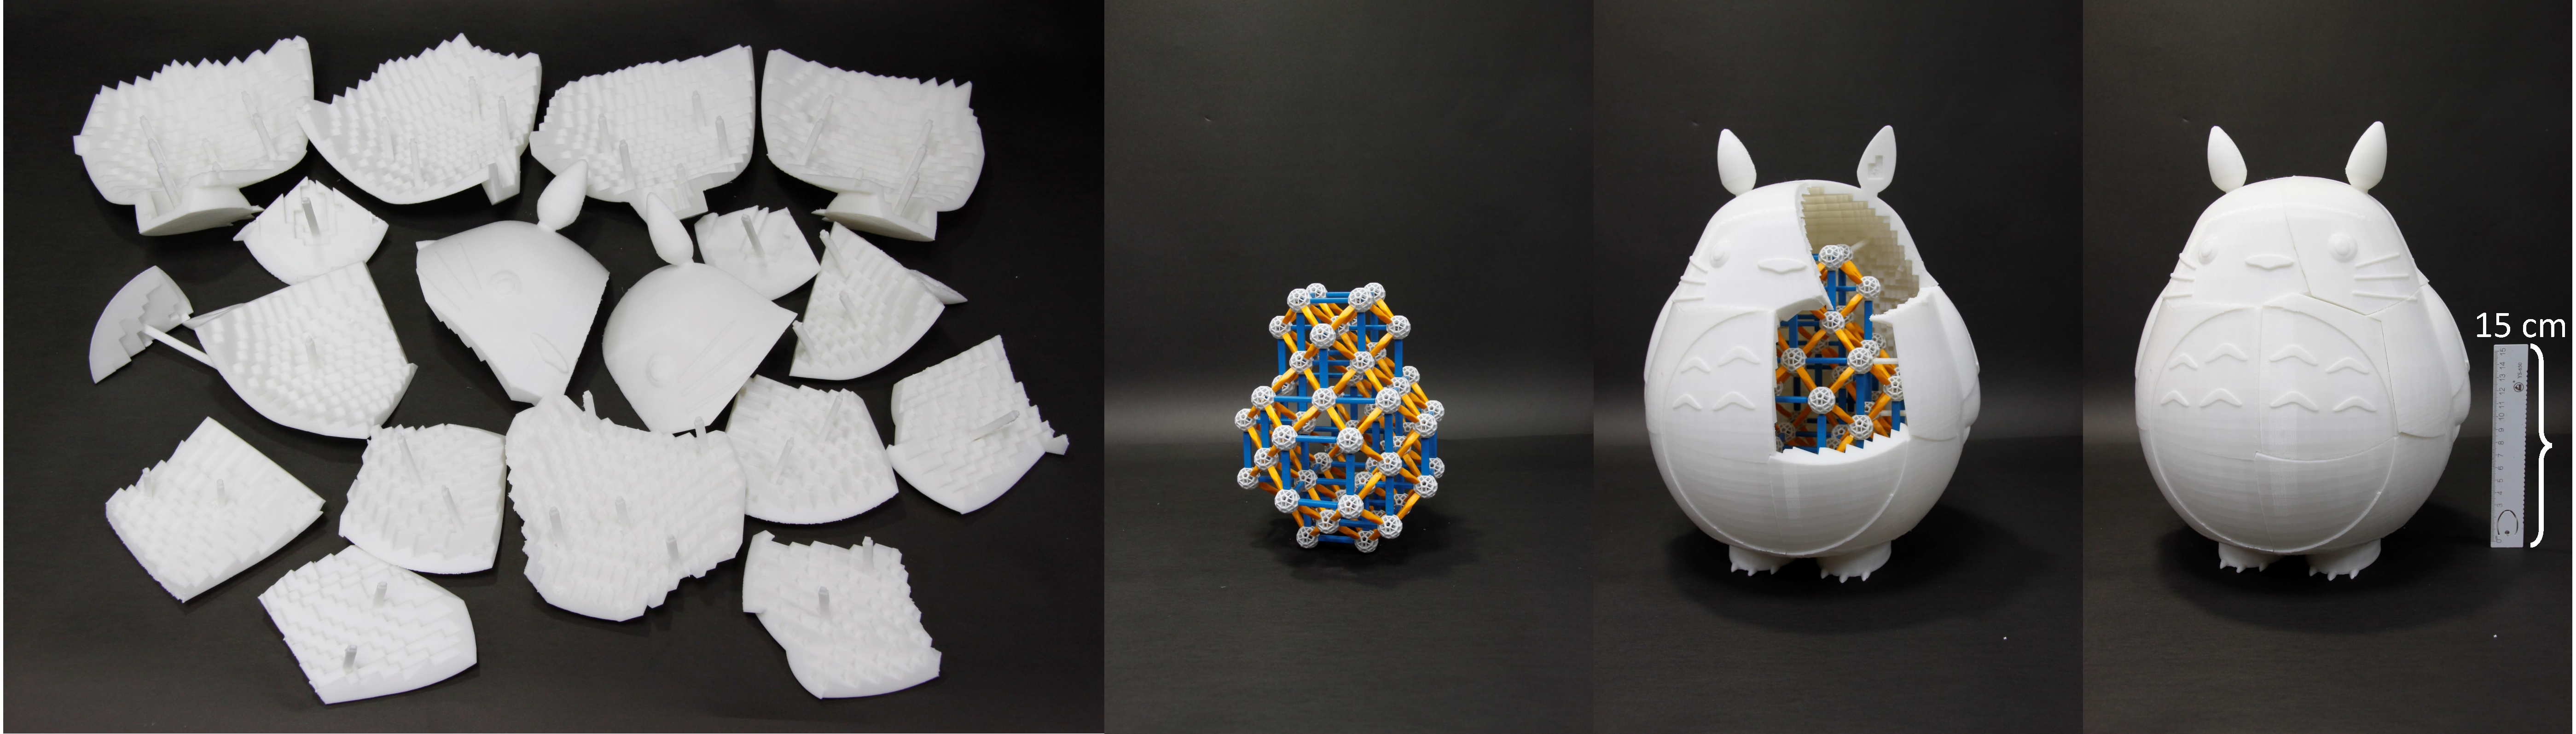
\includegraphics[width=1.0\linewidth]{figs/totoro_real.pdf} 
%\caption{Result fabricated and assembly : Totoro}
%\label{fig:result-assembly_doraemon_real}
%\end{figure*}

%\begin{figure*}[ht]
%\centering
%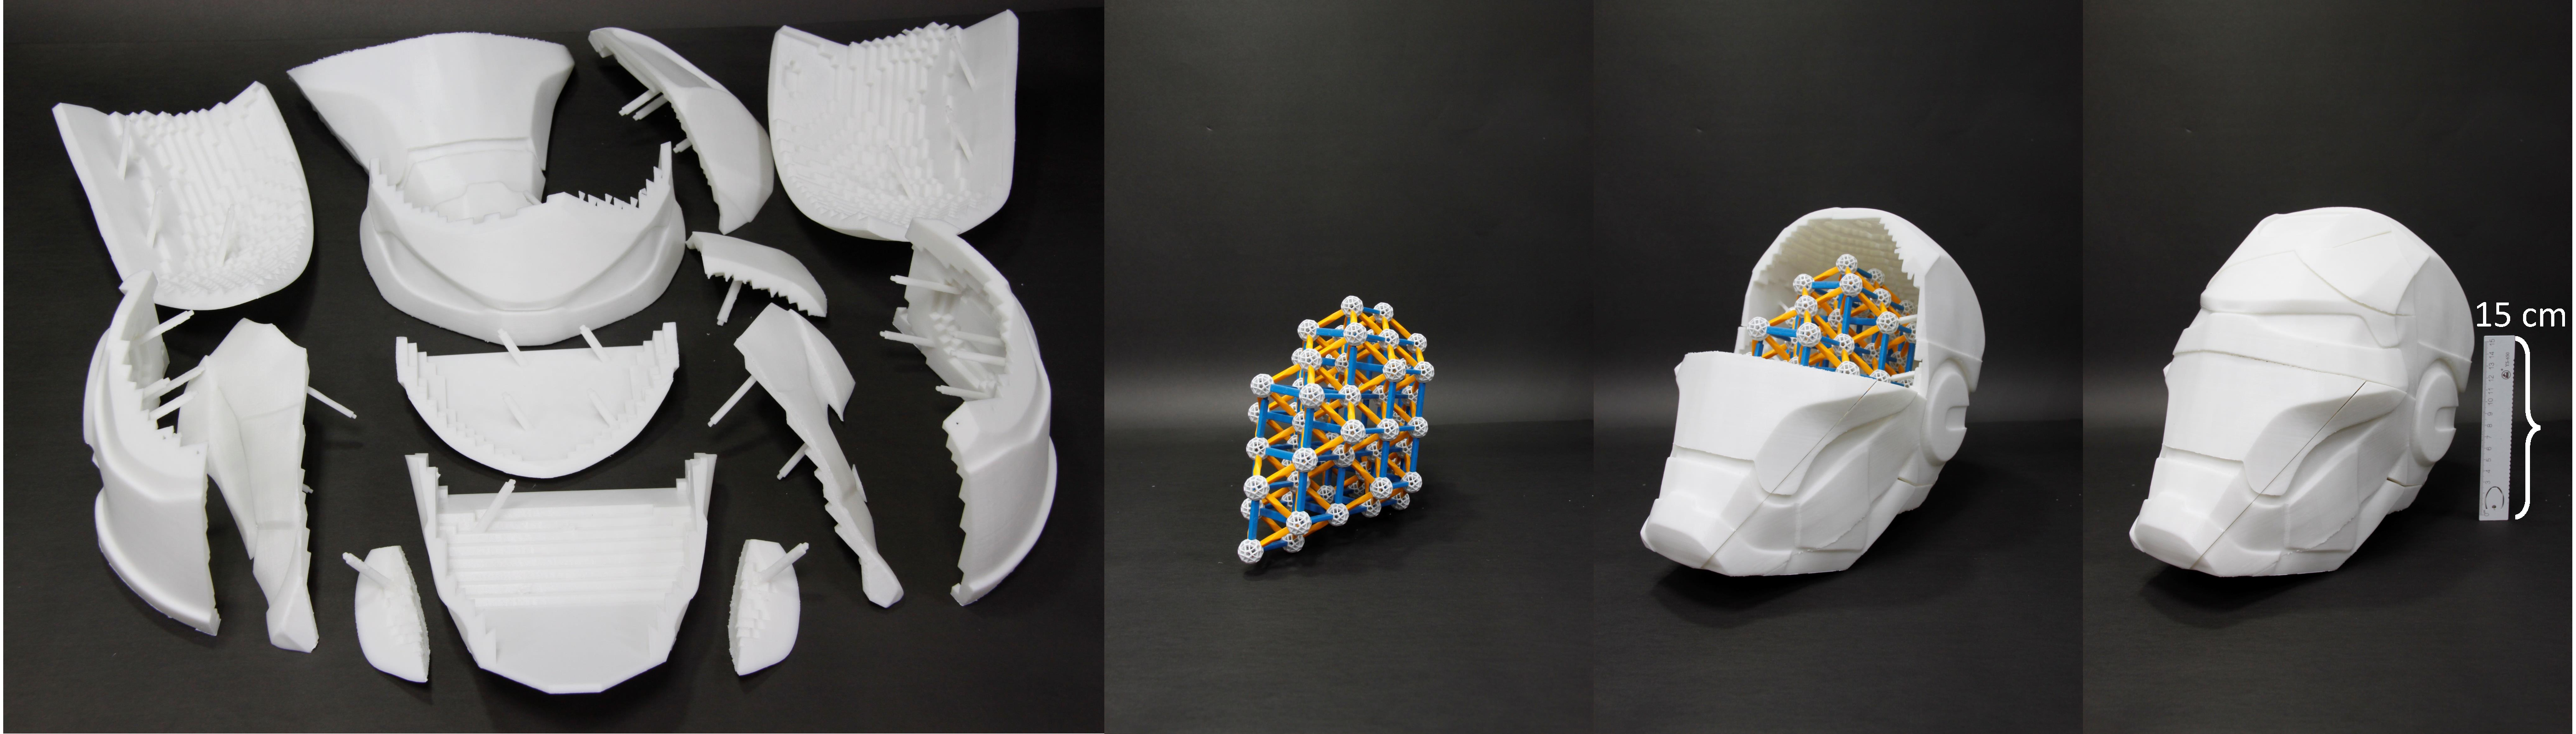
\includegraphics[width=1.0\linewidth]{figs/iron_real.pdf} 
%\caption{Result fabricated and assembly : Iron}
%\label{fig:result-assembly_doraemon_real}
%\end{figure*}

%\begin{figure*}[ht]
%\centering
%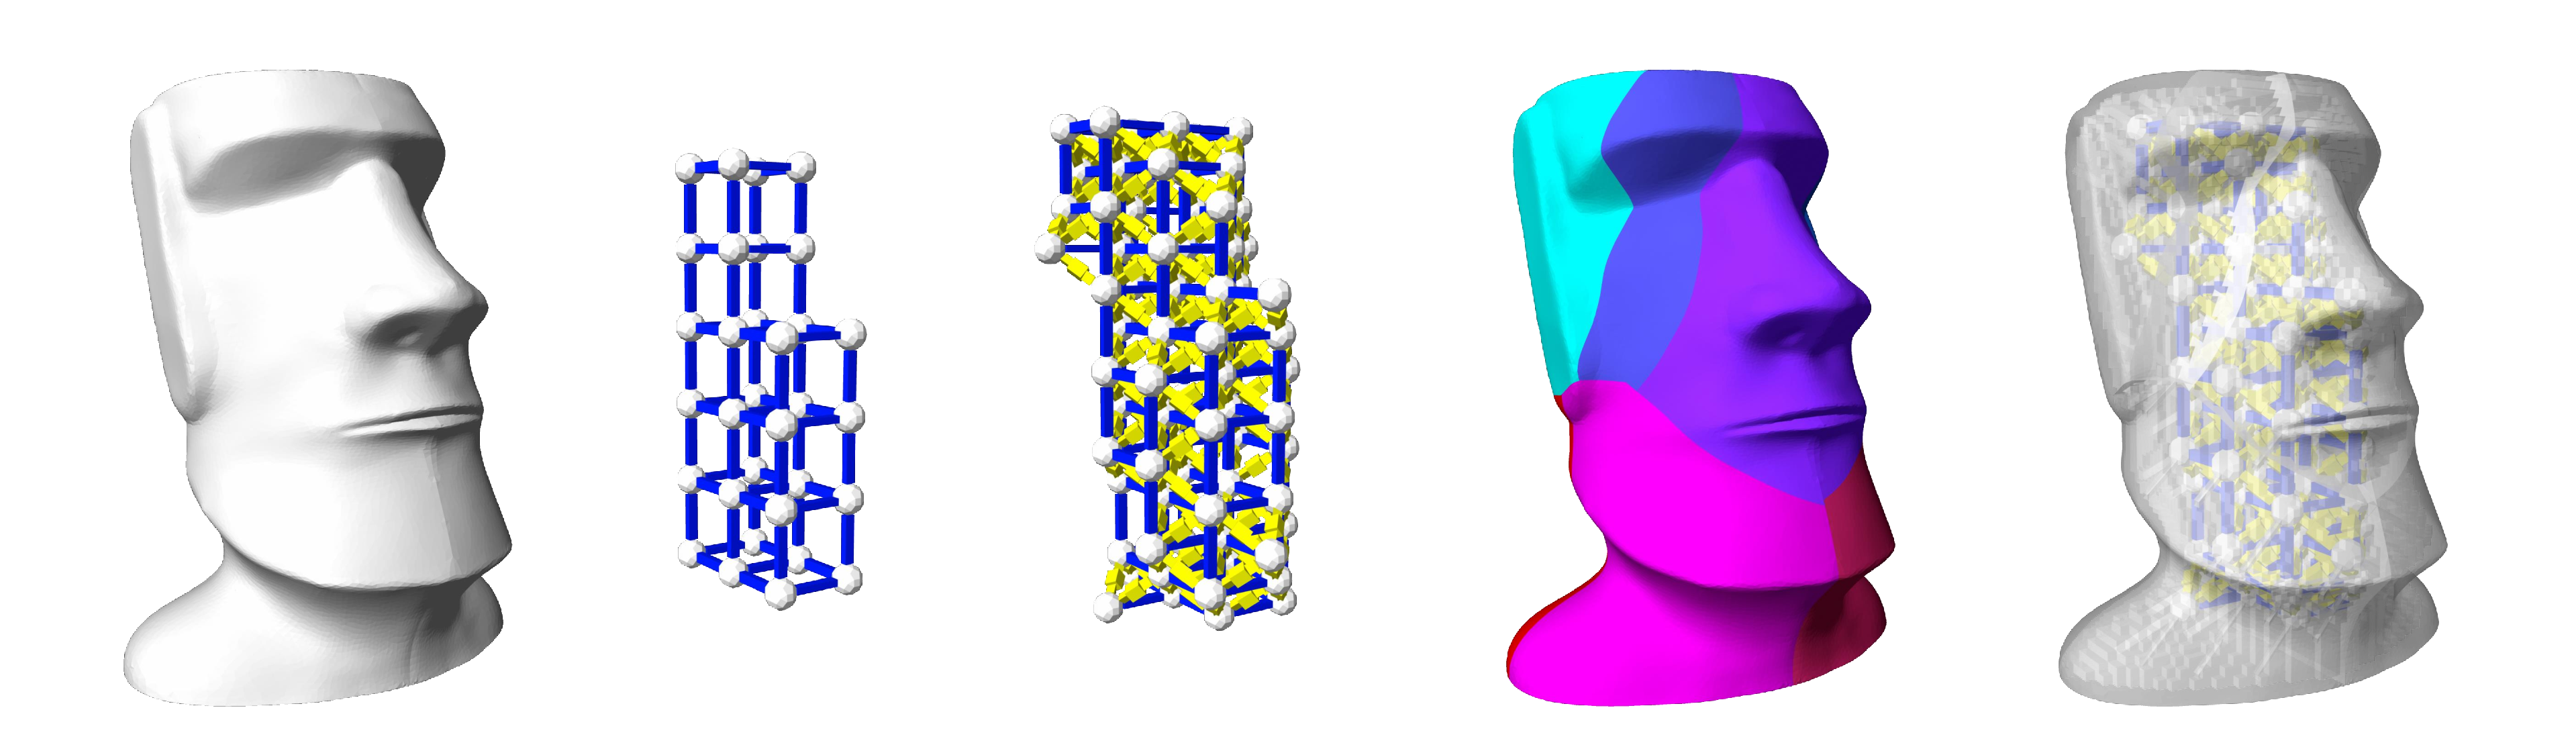
\includegraphics[width=1.0\linewidth]{figs/MOAI.pdf} 
%\caption{Result : MOAI}
%\label{fig:result-assembly_MOAI}
%\end{figure*}

%\begin{figure*}[ht]
%\centering
%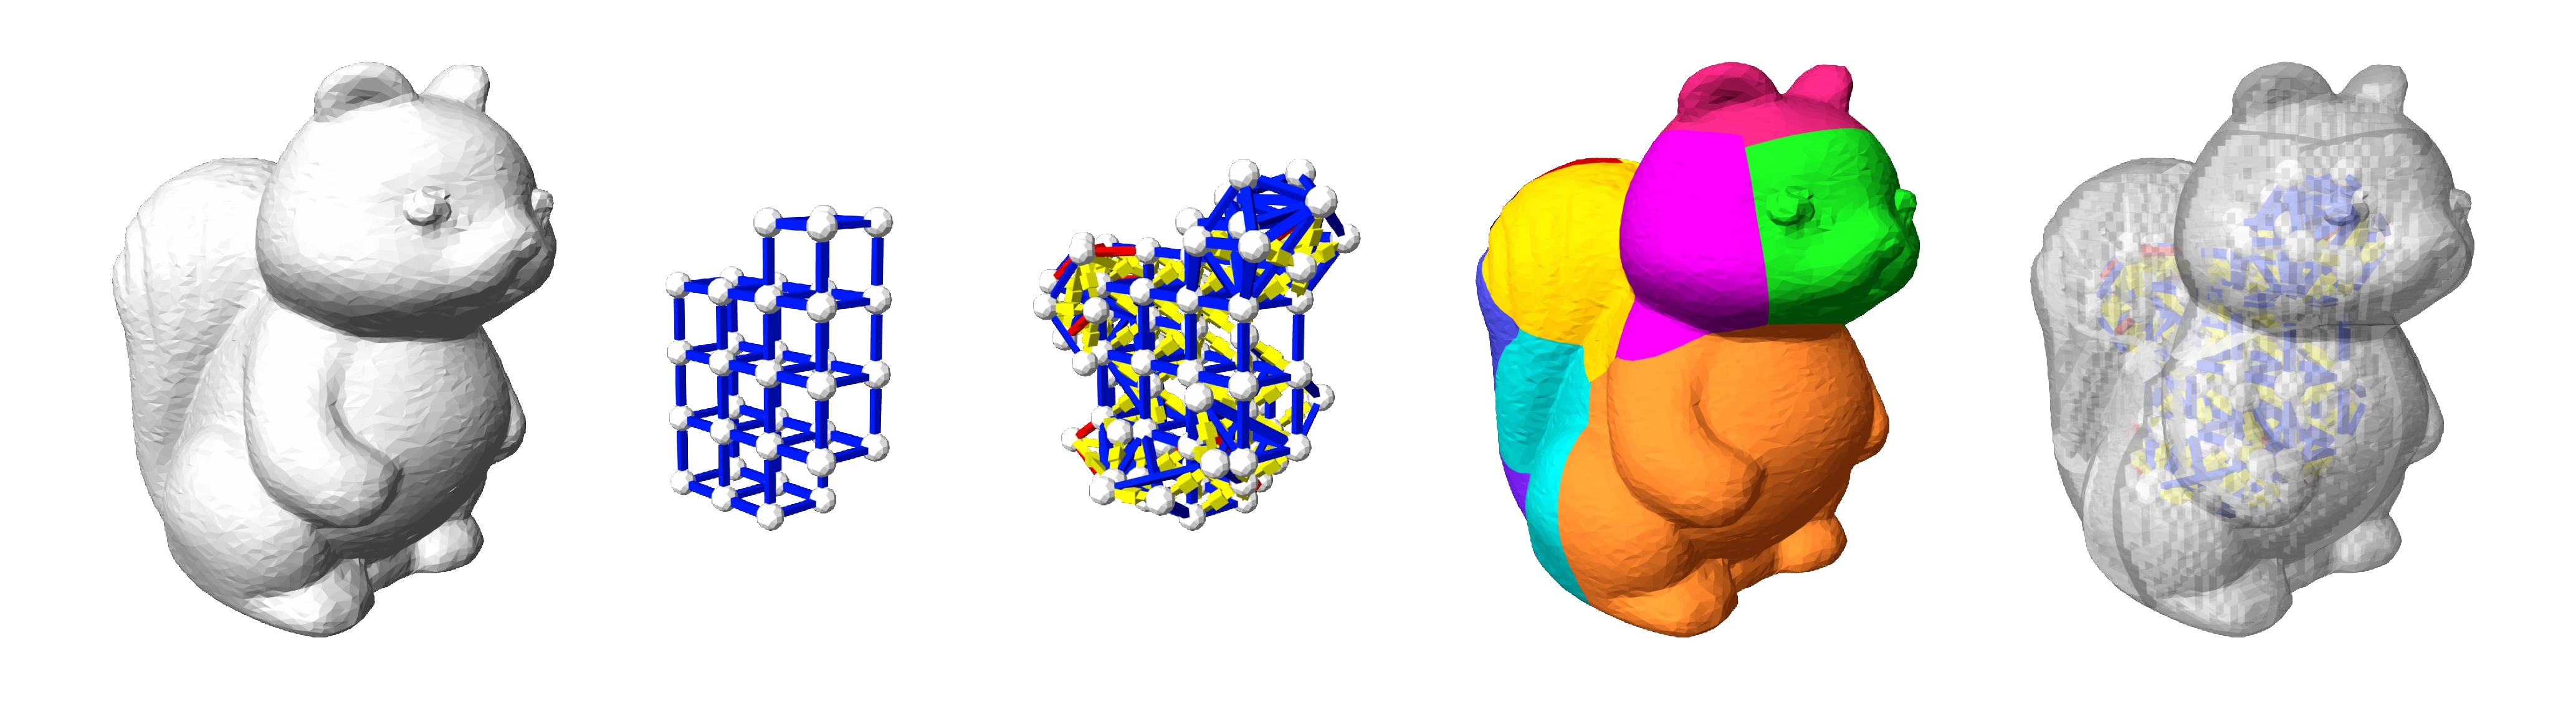
\includegraphics[width=1.0\linewidth]{figs/Squirrel.pdf} 
%\caption{Result : Squirrel}
%\label{fig:result-assembly_Squirrel}
%\end{figure*}

%\begin{figure*}[ht]
%\centering
%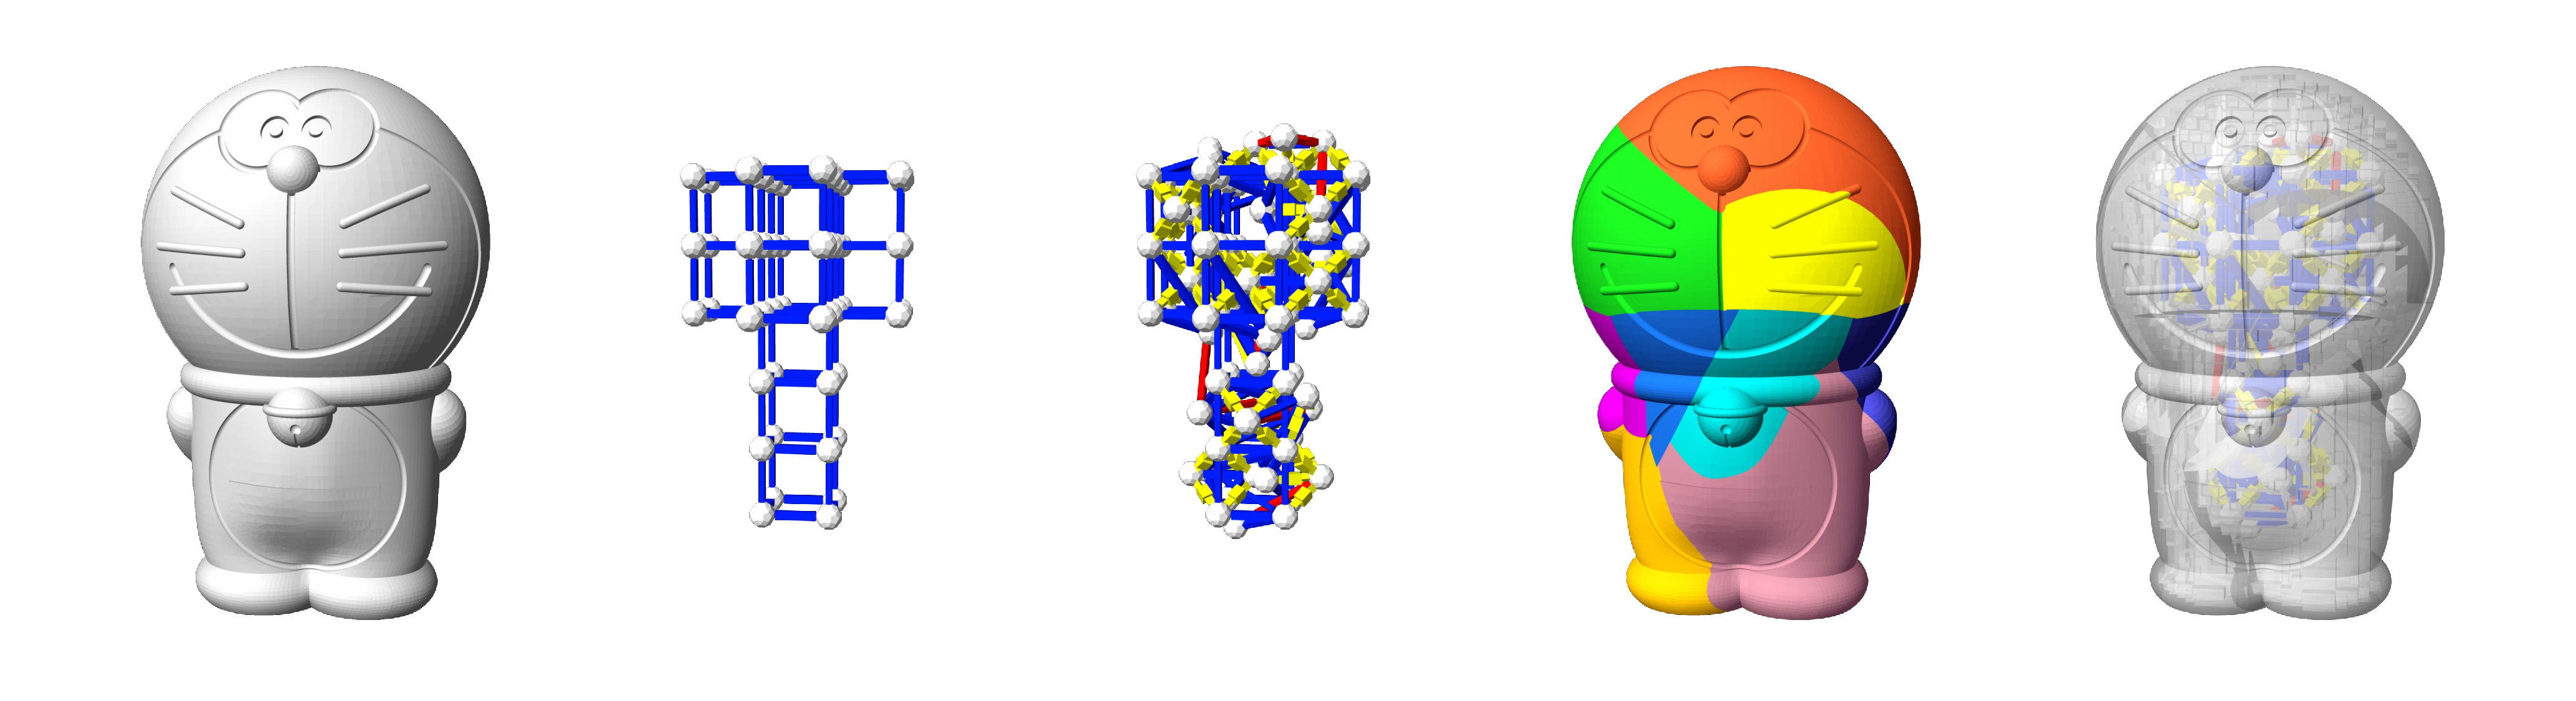
\includegraphics[width=1.0\linewidth]{figs/doraemon.pdf} 
%\caption{Result : Doraemon}
%\label{fig:result-assembly_doraemon}
%\end{figure*}

%\begin{figure*}[ht]
%\centering
%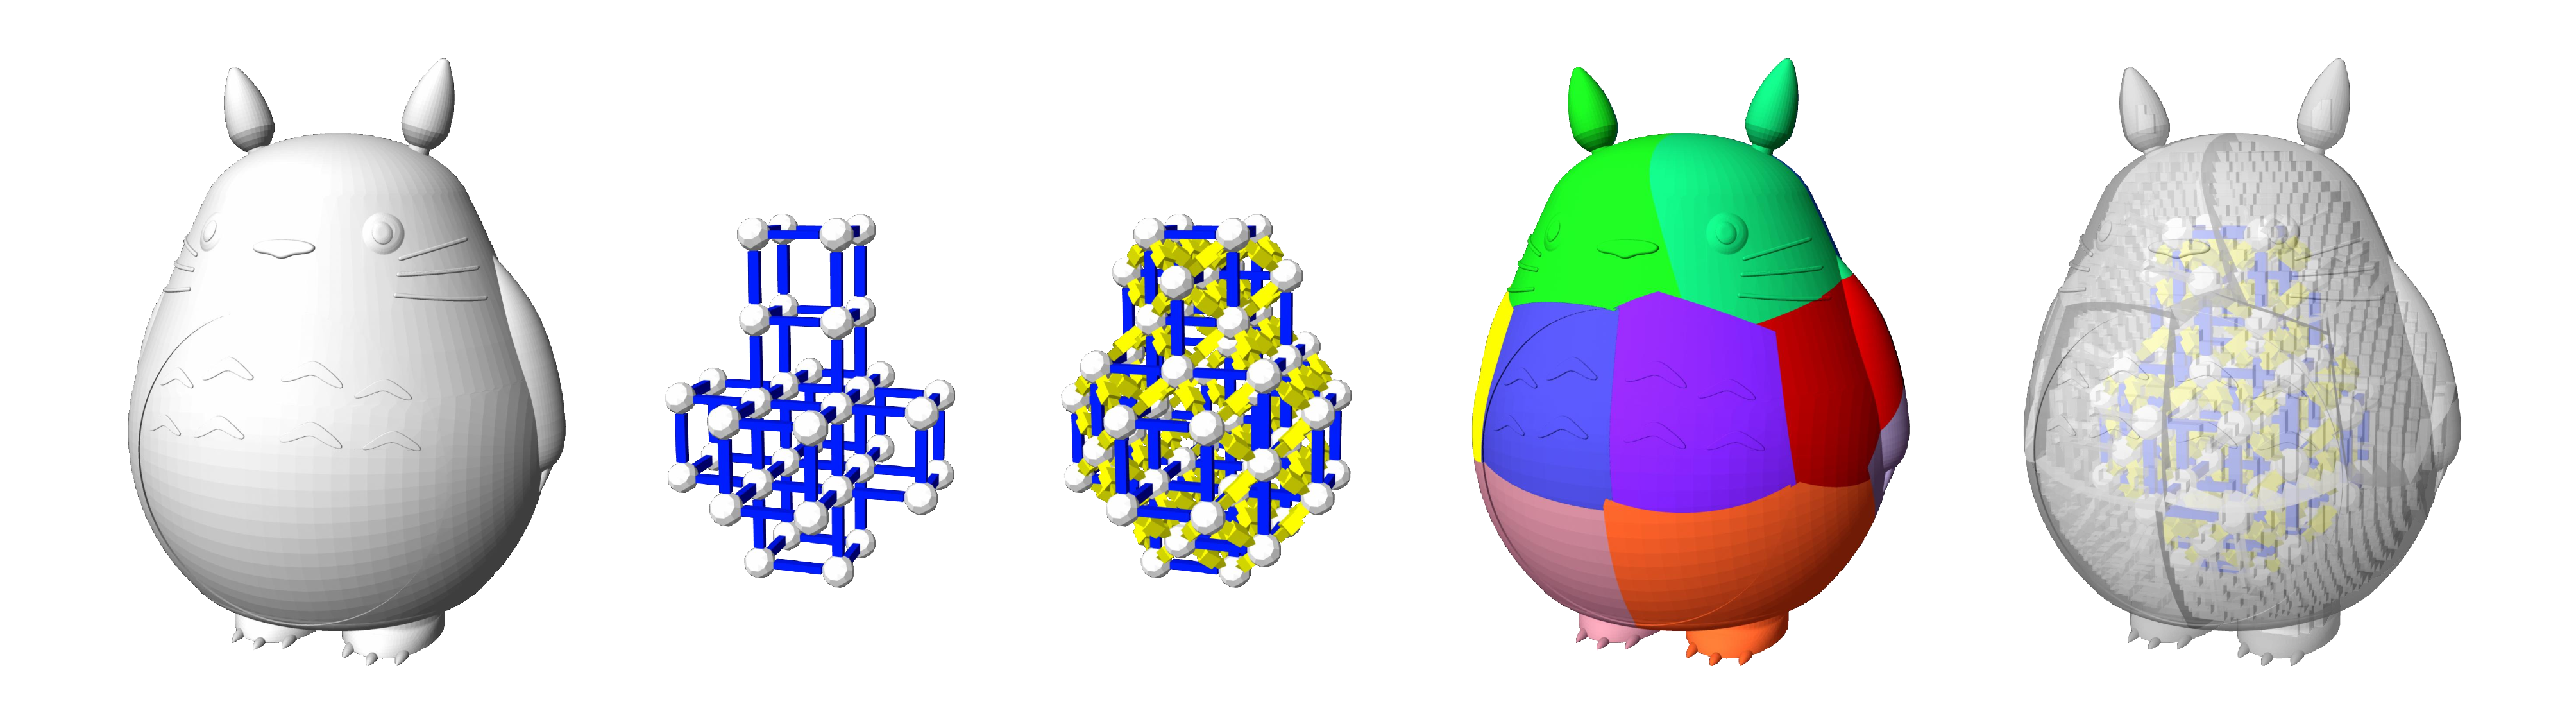
\includegraphics[width=1.0\linewidth]{figs/totoro.pdf} 
%\caption{Result : Totoro}
%\label{fig:result-assembly_totoro}
%\end{figure*}

%\begin{figure*}[ht]
%\centering
%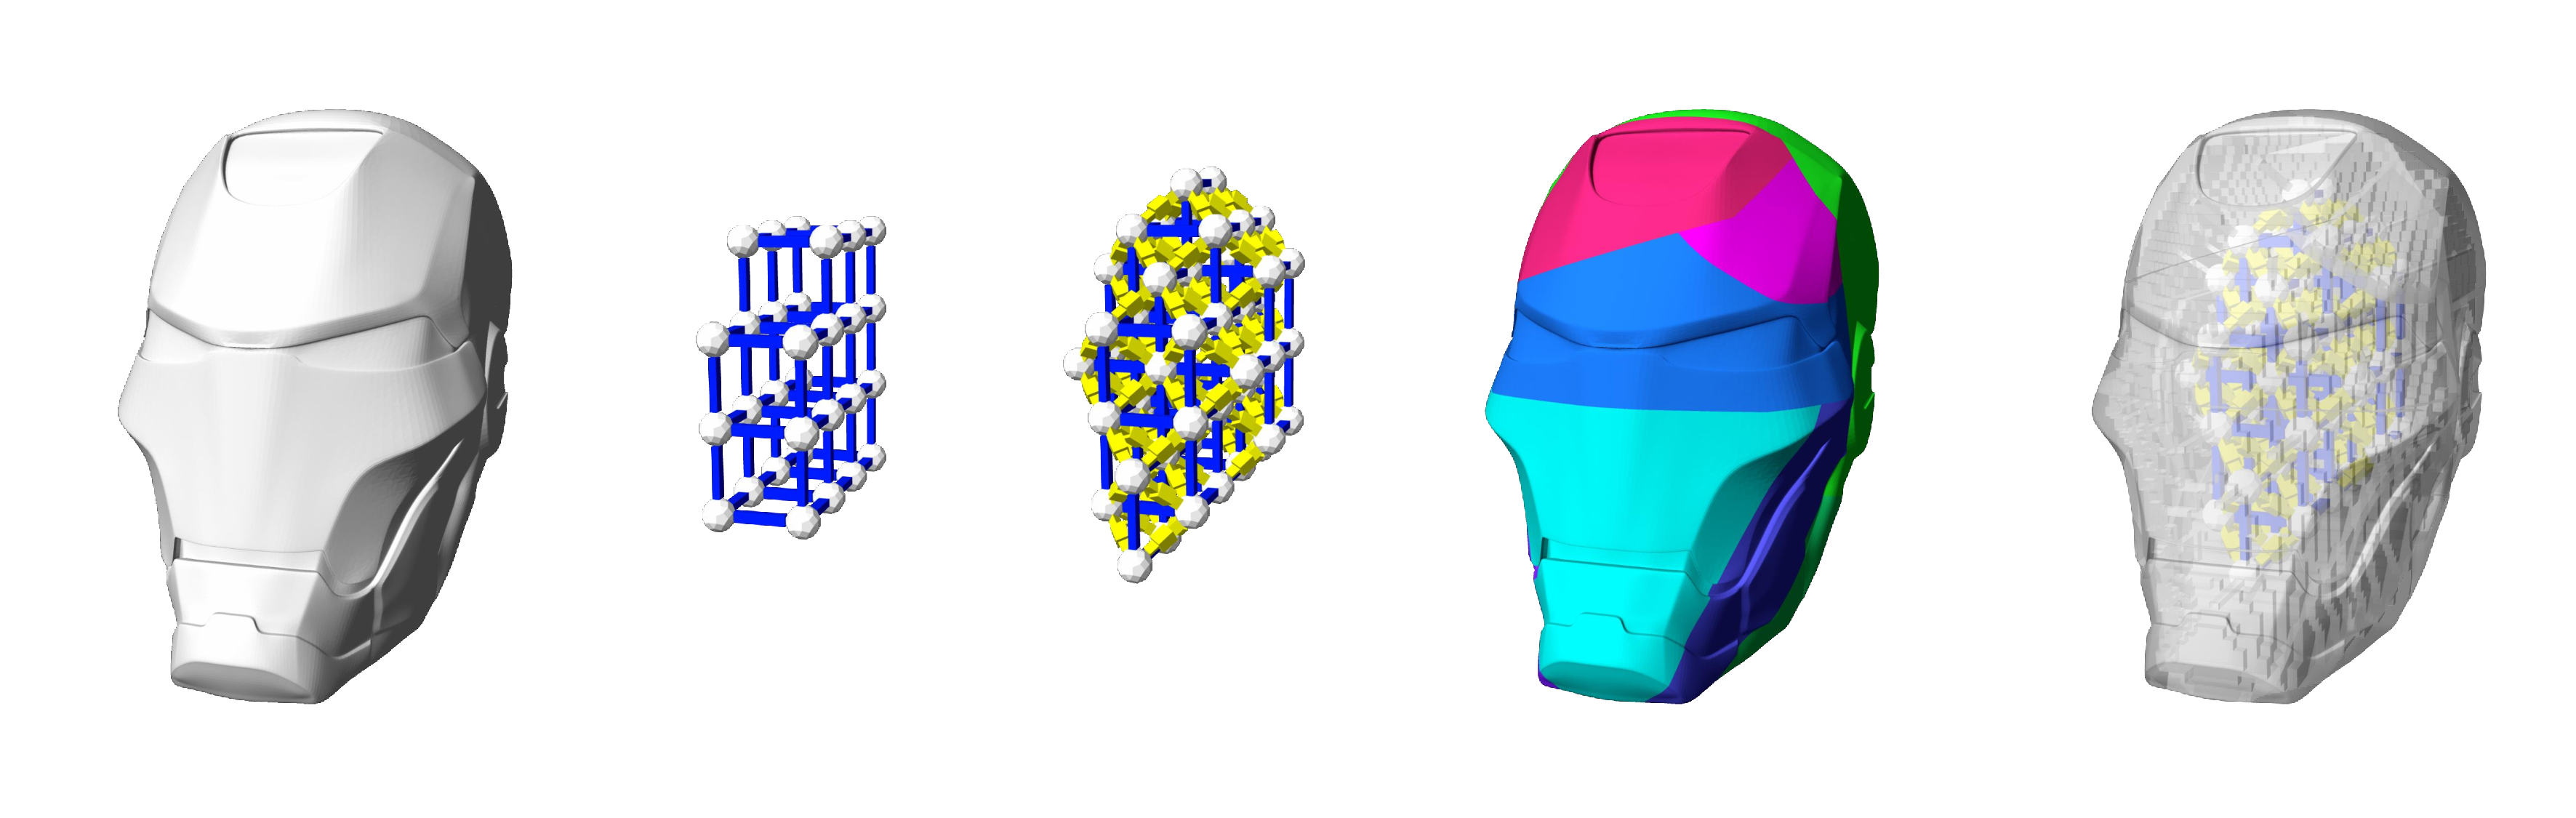
\includegraphics[width=1.0\linewidth]{figs/iron.pdf} 
%\caption{Result : Iron Man}
%\label{fig:result-assembly_iron}
%\end{figure*}

%\begin{figure*}[ht]
%\centering
%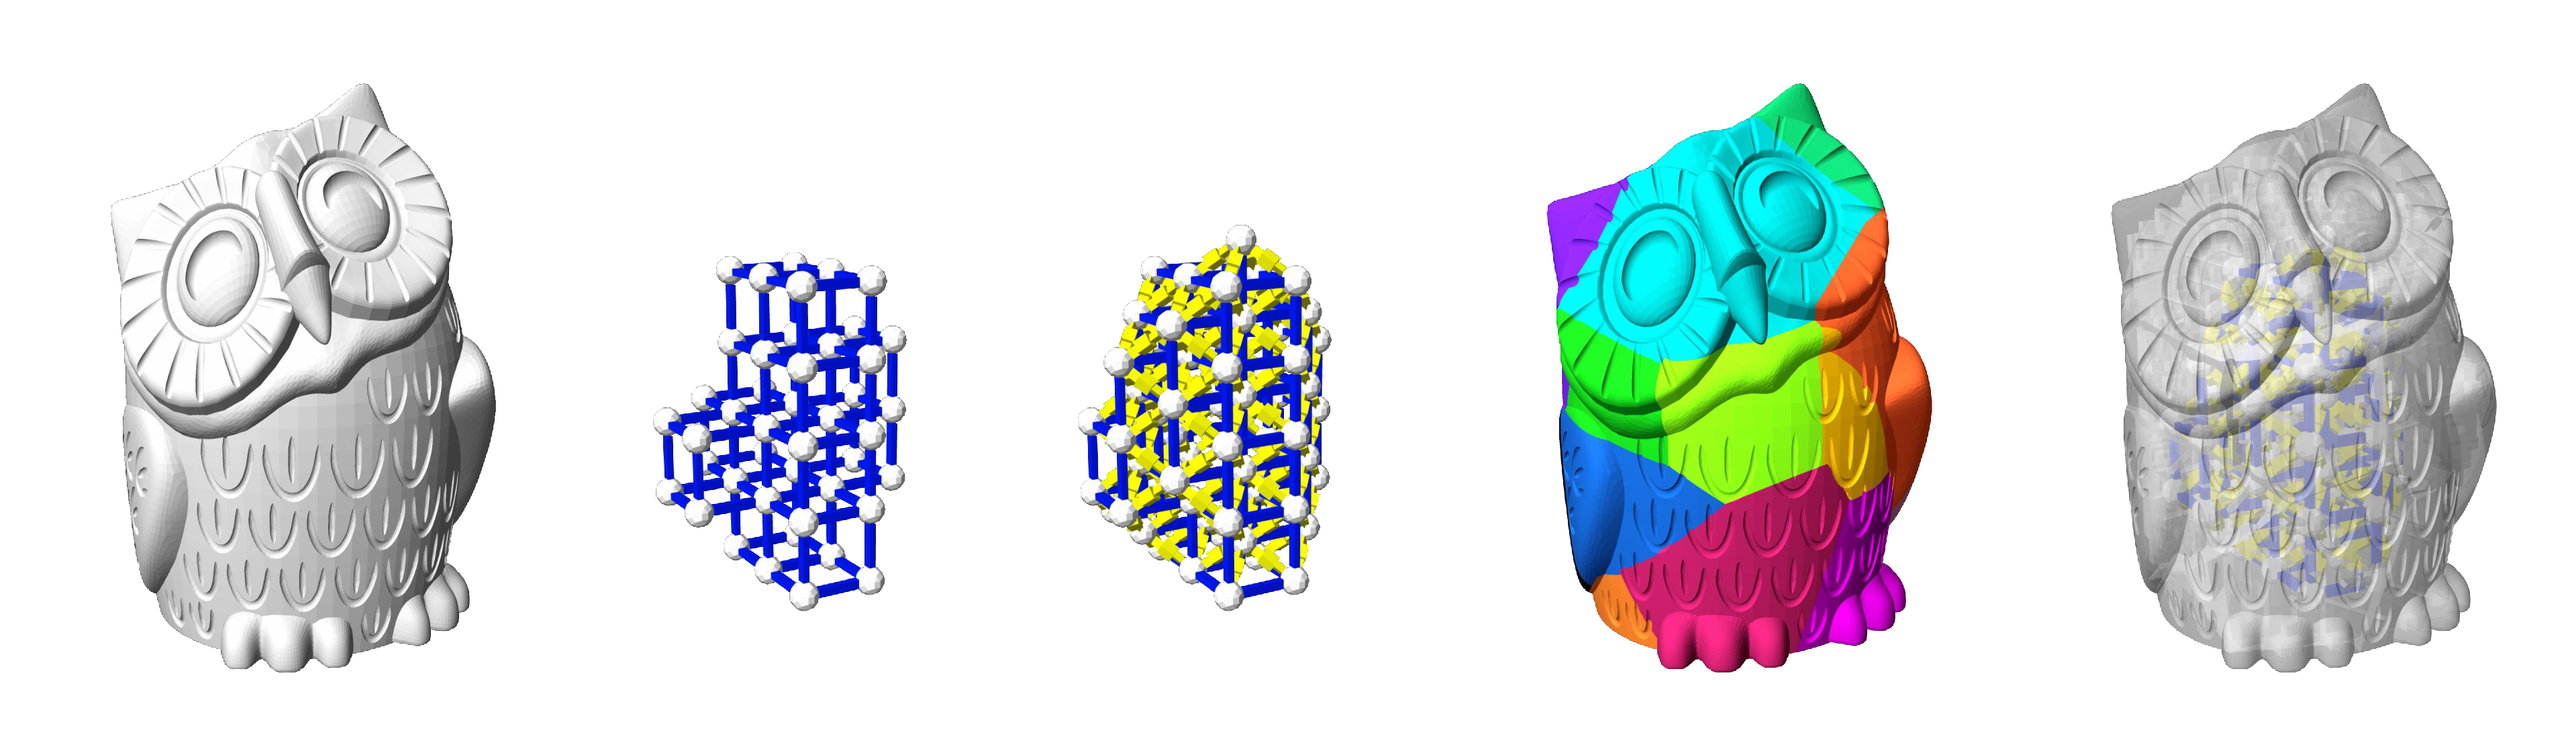
\includegraphics[width=1.0\linewidth]{figs/owl.pdf} 
%\caption{Result : Owl}
%\label{fig:result-assembly_owl}
%\end{figure*}

%\begin{figure*}[ht]
%\centering
%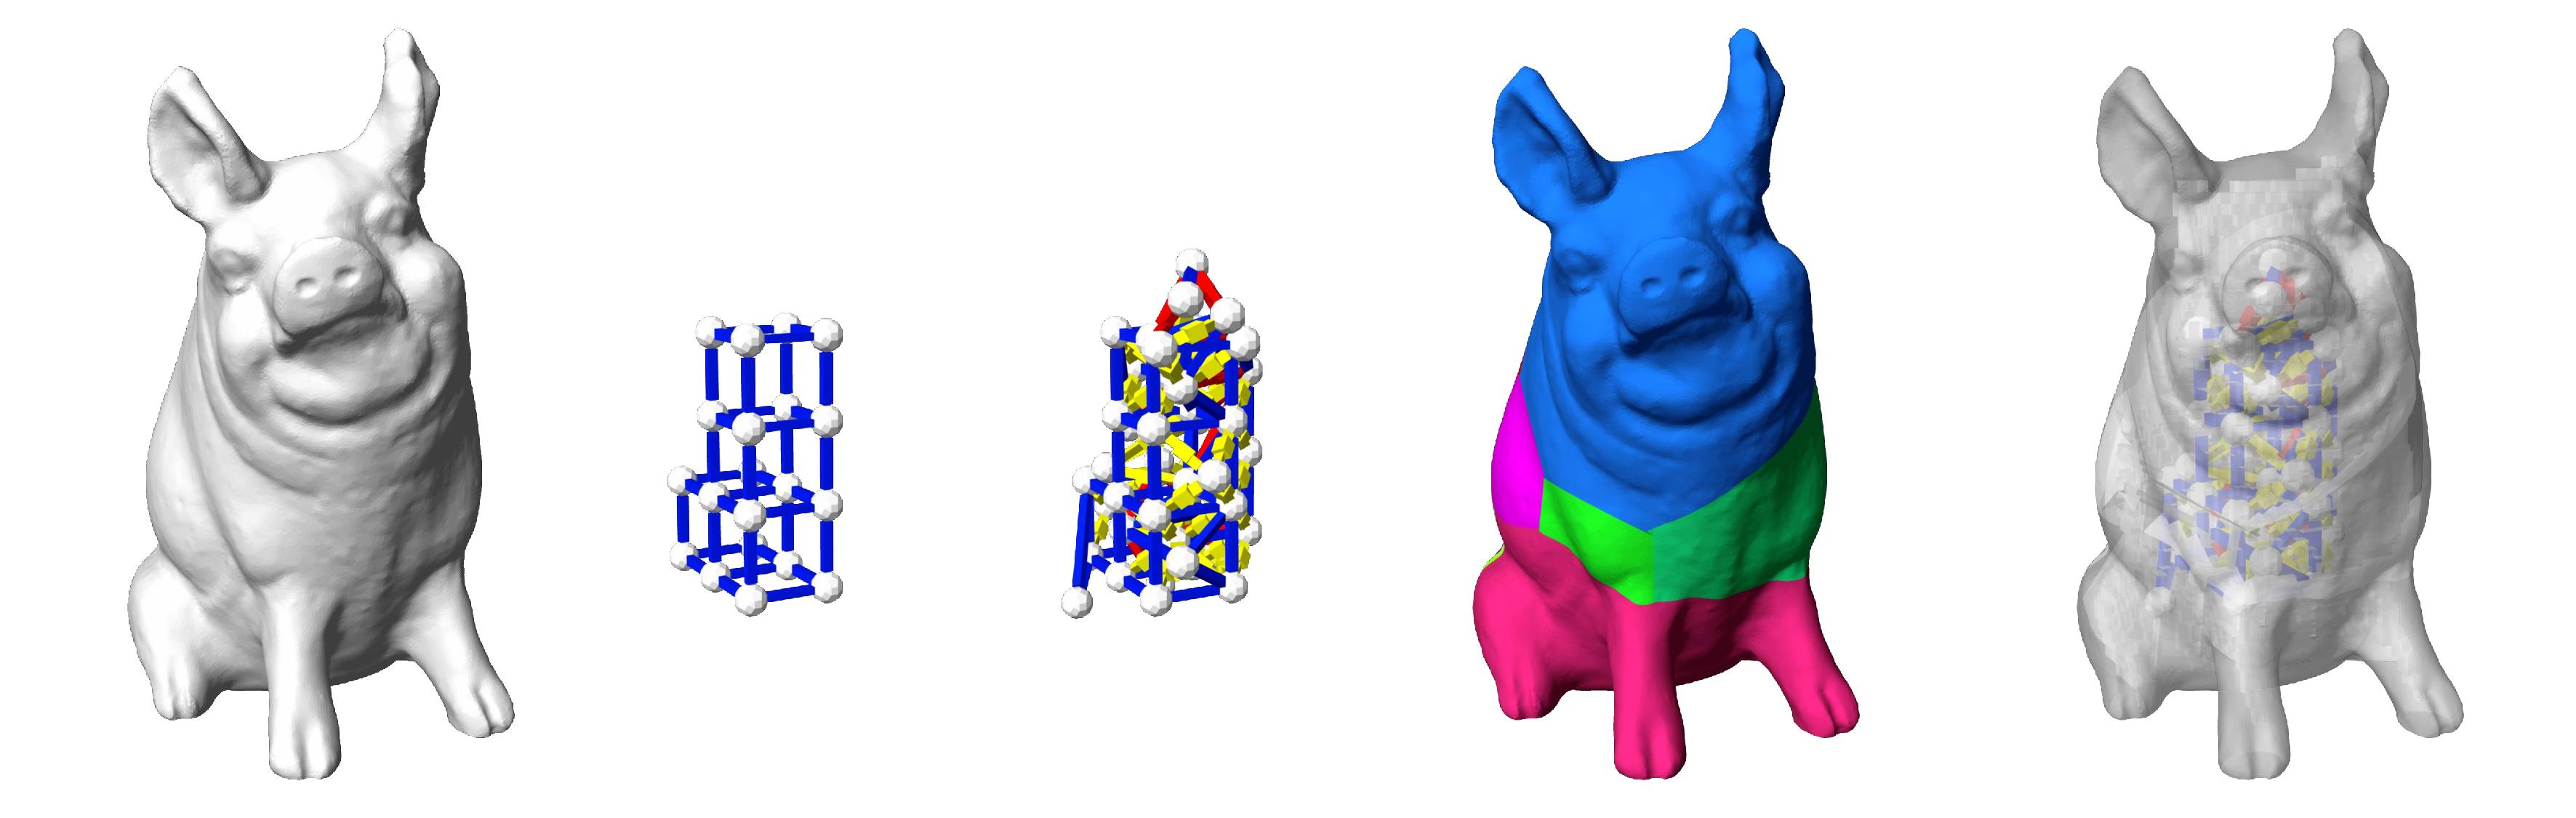
\includegraphics[width=1.0\linewidth]{figs/pig.pdf} 
%\caption{Result : Pig}
%\label{fig:result-assembly_pig}
%\end{figure*}

%\begin{figure*}[ht]
%\centering
%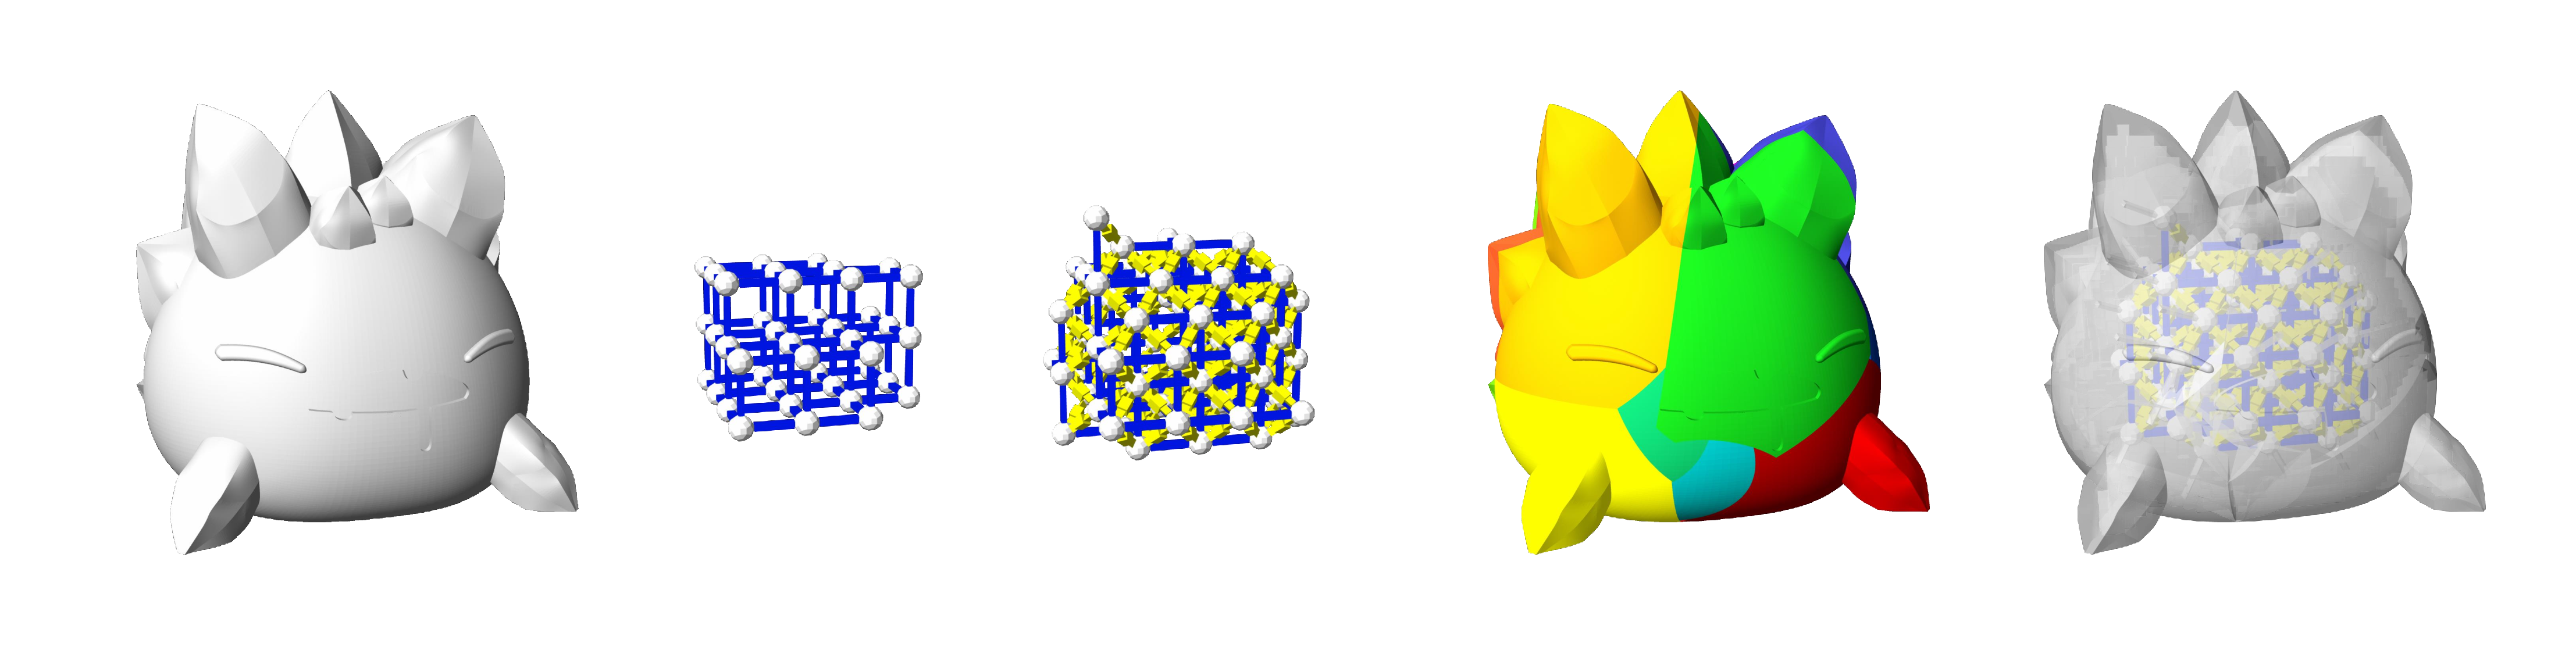
\includegraphics[width=1.0\linewidth]{figs/slime_high.pdf}
%\caption{Result : Slime}
%\label{fig:result-assembly_slime}
%\end{figure*}

%\begin{figure*}[ht]
%\centering
%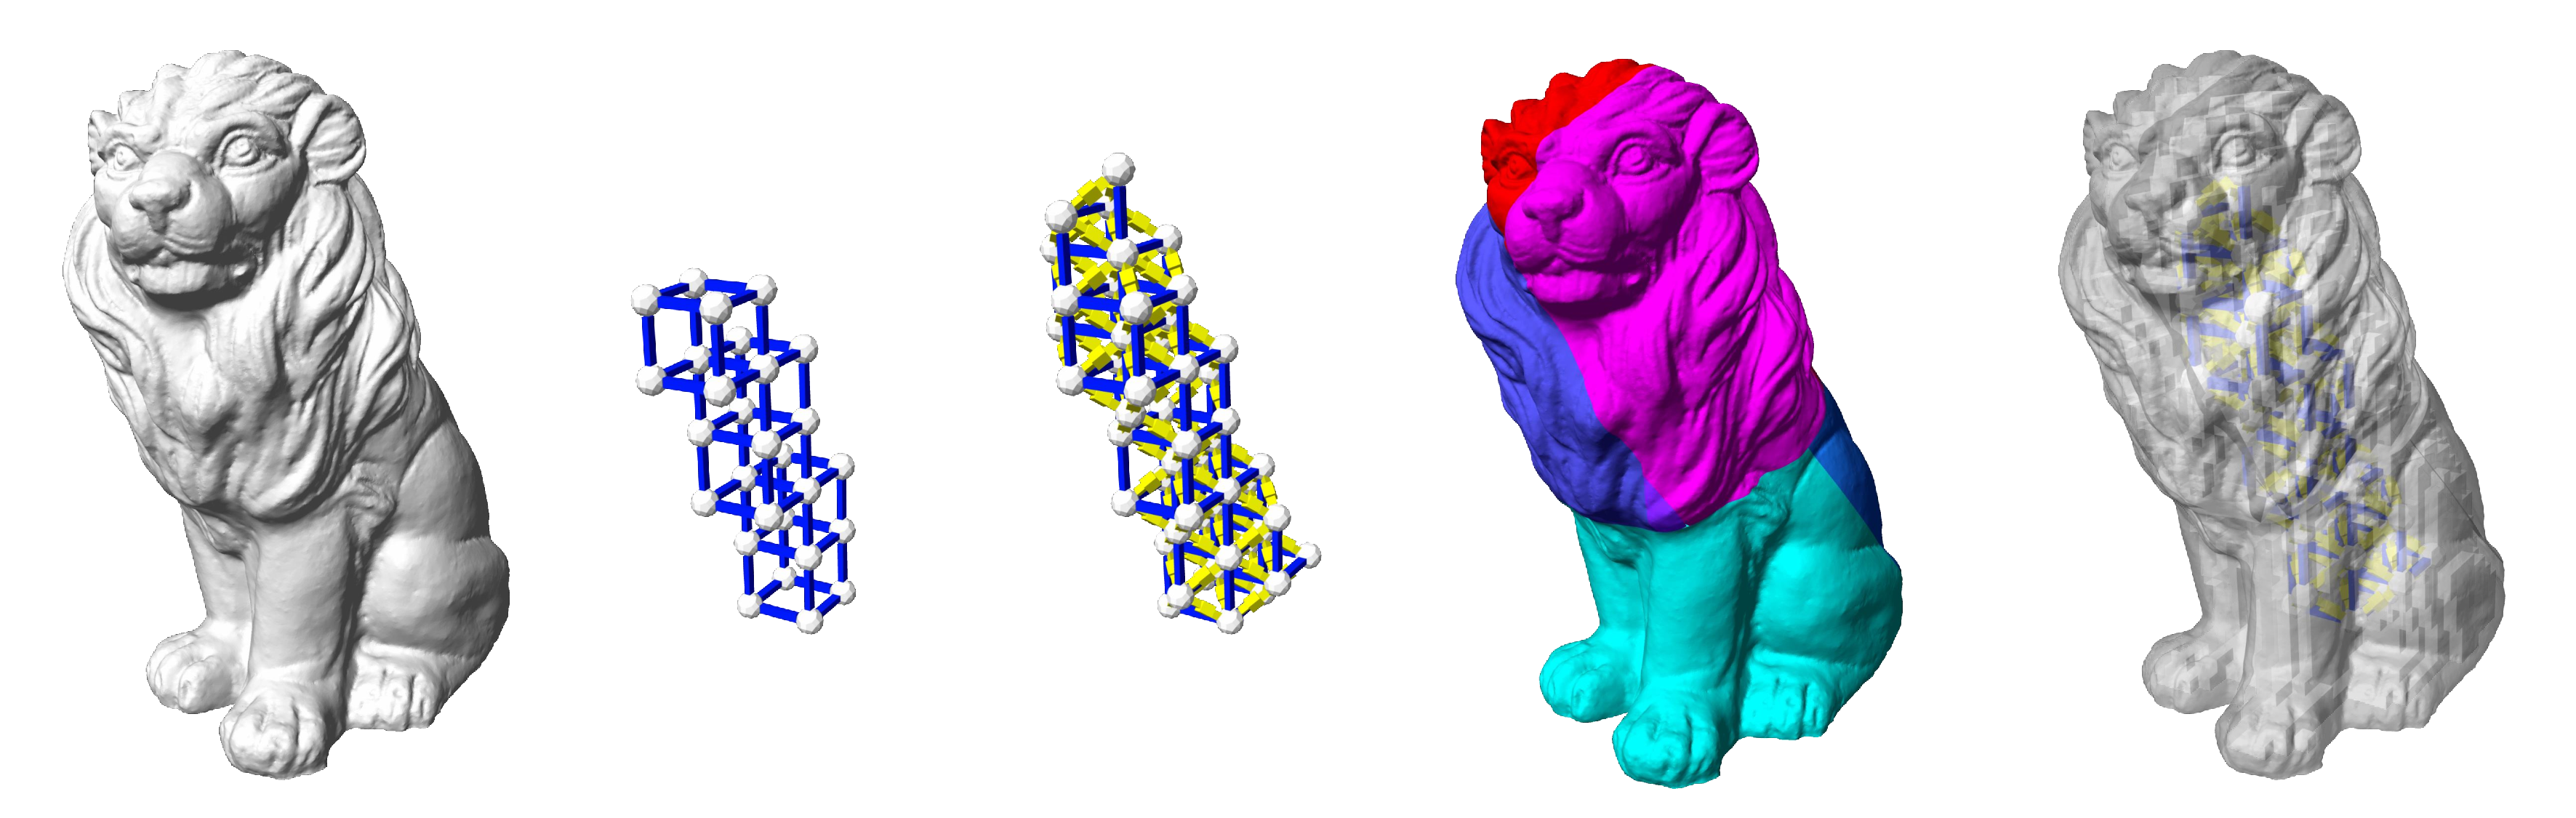
\includegraphics[width=1.0\linewidth]{figs/lion.pdf} 
%\caption{Result : Lion}
%\label{fig:result-assembly_lion}
%\end{figure*}

%\begin{figure*}[ht]
%\centering
%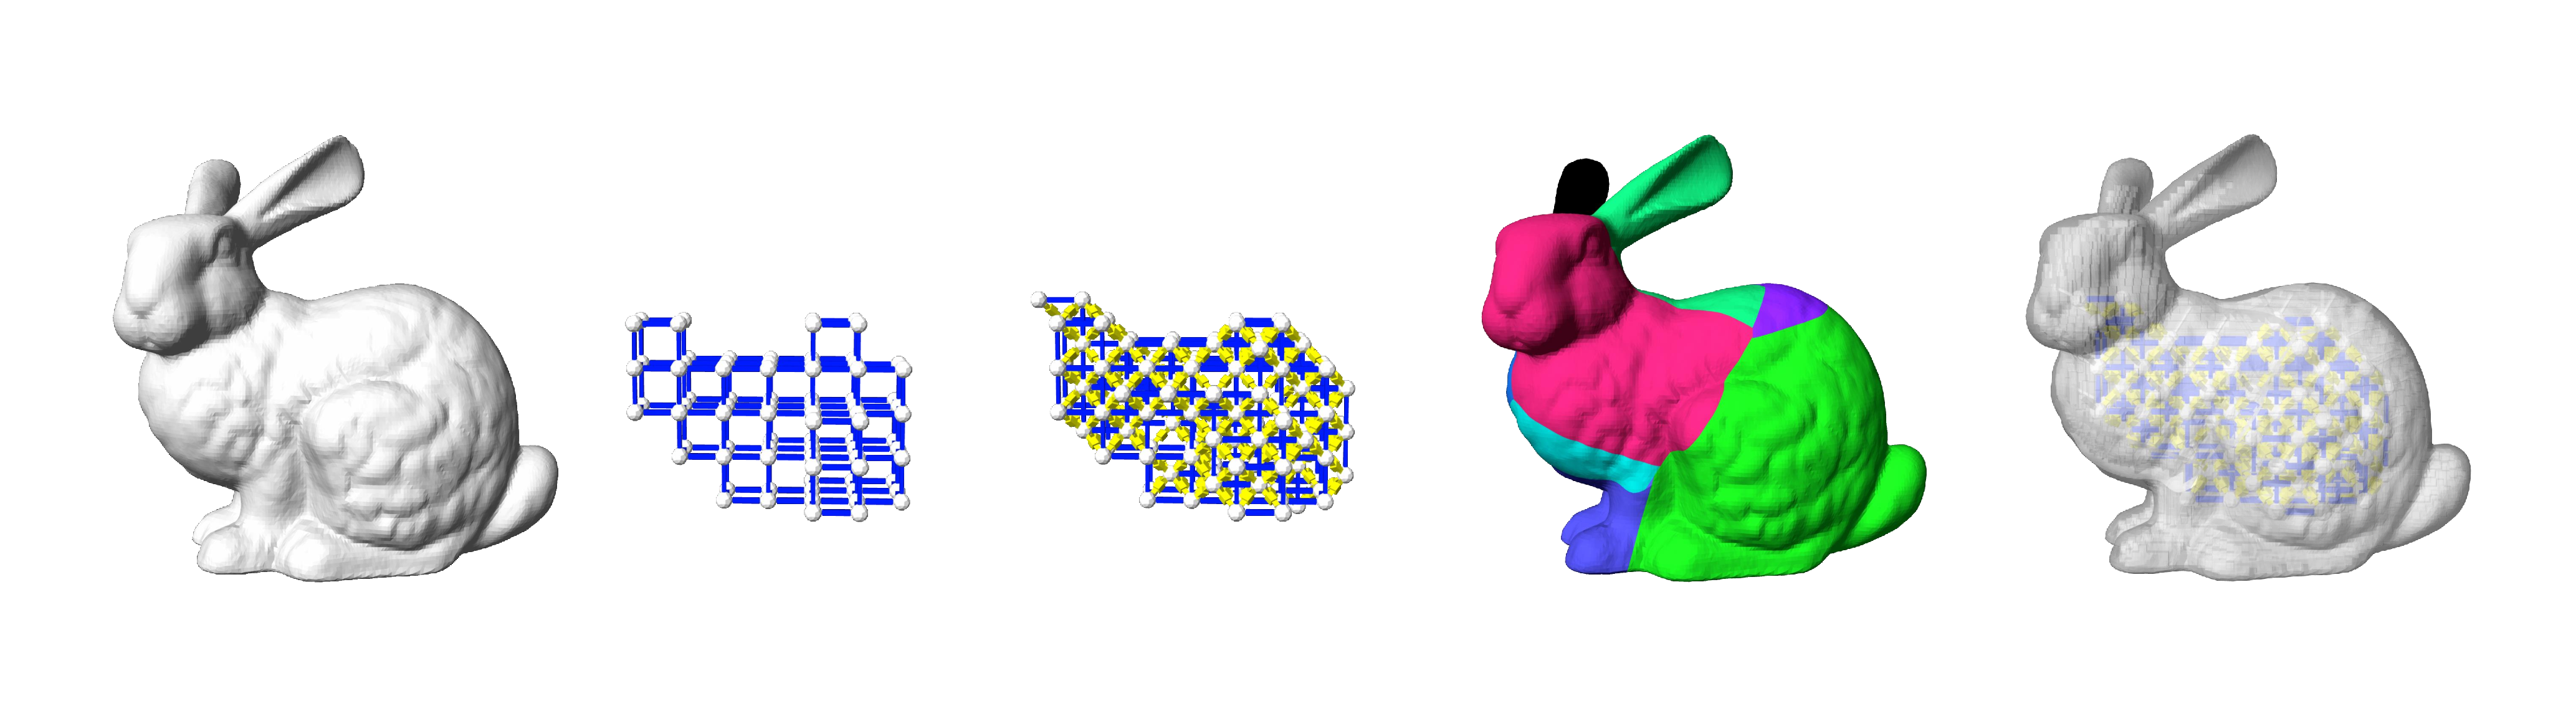
\includegraphics[width=1.0\linewidth]{figs/bunny_150.pdf} 
%\caption{Result : Bunny}
%\label{fig:result-assembly_Bunny}
%\end{figure*}
